% --------------------------------------------------------------------------
% This is a LaTeX template for a University of Idaho Master's thesis.
% It uses a custom document class file, UIdahoMastersThesis
% The class and template adhere to the formatting guidelines established by UI College of Graduate Studies (CoGS) as of 2016.
% That being said, DOUBLE CHECK everything, I'm not perfect, and this isn't either.
% I highly recommend getting it reviewed by the Writing Center and CoGS BEFORE you're finished writing. Seriously.
% --------------------------------------------------------------------------
% Author   Christopher Goes
% Email    goesc@acm.org    (Alternate: goes8945@alumni.uidaho.edu)
% --------------------------------------------------------------------------
% This template (and my thesis!) would not be possible without the work of these awesome people.
%     - Matthew Brown, CS       For sharing his thesis and all the neat hacks it had
%     - Cara Leatherman, CoGS   For template improvements
%     - Chris Zeoli, CoGS       For the original UI CoGS template
% --------------------------------------------------------------------------

% This includes the magical class file with the formatting. ** DO NOT REPLACE THIS. Everything WILL break. **
\documentclass{UIdahoMastersThesis}

% --------------------------------------------------------------------------
% Packages (the class file already imports several. Importing twice usually doesn't hurt, just keep in mind for debugging)
\usepackage{rotating}
\usepackage[T1]{fontenc}
\usepackage{lmodern}
\usepackage{siunitx}
\sisetup{separate-uncertainty}% siunit setup
\sisetup{free-standing-units}%
\sisetup{round-minimum = 0.01}%
\usepackage{wasysym}
\usepackage{textcomp}
\usepackage{gensymb}
\usepackage[utf8]{inputenc}
\usepackage[document]{ragged2e} %allows for left alignment
\usepackage{parskip}
\usepackage{float} %allows graphics to stay where you want them
\usepackage{booktabs} %allows for better tables
\usepackage[flushleft]{threeparttable} %allows for specific table parts
\usepackage[backend=biber,
style=authoryear,
language=american,
citestyle=authoryear-comp,
dashed=false,
autocite=inline,
uniquename=false,
firstinits=true,
mincitenames= 1, maxcitenames=2,
maxbibnames=99, minbibnames=99]{biblatex}
\renewbibmacro{in:}{
\ifentrytype{article}{}{\printtext{\bibstring{in}\intitlepunct}}}
\DeclareNameAlias{default}{last-first}
\addbibresource{af_thesis_refs.bib}
\setlength{\RaggedRightParindent}{\parindent}
\makeatletter  % ** DO NOT REMOVE THIS ** (Actually, remove it, compile, and enjoy the stream of errors. Its beautiful :) )
\newcommand{\M}[1]{\multicolumn{1}{l}{#1}} %shorthand way to make a left-aligned multicolumn in a table
\newcommand{\C}[1]{\multicolumn{1}{c}{#1}} %shorthand way to make a centered multicolumn in a table

% --------------------------------------------------------------------------
% Thesis Information
\author{Austin N. Fife}
\thesisdegree{Master of Science}  % e.g Master of Science, Master of Engineering, etc.
\major{Entomology}  % e.g Computer Science, Computer Engineering, etc.
\advisor{Erik J. Wenninger, Ph.D.}  % Make sure title of names matches CoGS format requirements!
\cmone{Nilsa A. Bosque-Pérez, Ph.D.}  % First committee member (Alphabetical order by last name, if I recall correctly)
\cmtwo{Richard Novy, Ph.D.}  % Second committee member
\cmthree{Arash Rashed, Ph.D.}  % Third committee member
\deptadmin{Edwin Lewis, Ph.D.}  % Department administrator or chair
\graddate{December, 2018}  % Graduation date, e.g May, 2017
% --------------------------------------------------------------------------

% Line spacing. The University of Idaho requires thesis formatting to be 1.5-2.0. In LaTeX 1.3=1.5, 1.6=2.0.
\linespread{1.5}

% Defines section counter for frontmatter. This way section number does not appear in the TOC for frontmatter sections
\setcounter{secnumdepth}{0}

% Sets what level of sections show up in the table of contents. 0 = sections, 1 = subsections, 2 = subsubsections, etc.
\setcounter{tocdepth}{1}


% Configure the PDF output (Most of this is optional, it just adds metadata to the PDF)
\usepackage[% pdftex
pdfauthor=\author,
pdftitle={Investigating behavior of the potato psyllid Bactericera cockerelli (Šulc) (Hemiptera: Triozidae) on three potato genotypes with putative resistance to “Candidatus Liberibacter solanacearum”},
pdfsubject={Entomology},
pdfkeywords={Bactericera cockerelli;Solanum tuberosum;Candidatus Liberibacter solanacearum;Entomology;psyllid},
pdfproducer={ShareLatex},  % e.g ShareLatex
pdfcreator={pdflatex},
pdfprintscaling={AppDefault}]
{hyperref}

% Configure hyperlinks
\hypersetup{
	colorlinks=true, %set true if you want colored links
	linktoc=all,     %set to all if you want both sections and subsections linked
	linkcolor=black,  %choose some color if you want links to stand out
	citecolor=black,
	urlcolor=black,
}

% Changes default indenting in list of figures to 0
%\makeatletter
\renewcommand*\l@figure{\@dottedtocline{1}{0em}{2.3em}}% Default: 1.5em/2.3em
\let\l@table\l@figure
%\makeatother

% Where to look for images
% (https://en.wikibooks.org/wiki/LaTeX/Importing_Graphics#Graphics_storage)
\graphicspath{ {./Figures/} }

% Uncomment to set default style for Listings to be code (Code style is defined in .cls file)
% \lstset{style=code}

% -------------------------------------------------------------------------
\begin{document}
\frontmatter

\titleformat{\chapter}[block]{\scshape\LARGE}{\centering\chaptertitlename\ \thechapter:}{1ex}{\centering}{}
	\titlespacing{\chapter}{0pt}{-40pt}{20pt}

\titleformat{\section}[hang]{\scshape\Large}{\thesection}{1ex}{}
    \titlespacing{\section}{0pt}{0pt}{10pt}
	%\titlespacing*{\section}{0pt}{-50pt}{40pt}

\titleformat{\subsection}[hang]{\scshape\large}{\thesubsection}{1ex}{}
    \titlespacing{\subsection}{0pt}{0pt}{10pt}
	%\titlespacing*{\subsection}{0pt}{-50pt}{40pt}


% -------------------------------------------------------------------------
% -- Title Page --
\thesistitlepage


% --------------------------------------------------------------------------
% -- Authorization to Submit Thesis --
\frontmattersection{Authorization to Submit Thesis}
\authorizationpage
\newpage


% --------------------------------------------------------------------------
% -- Abstract --
\frontmattersection{Abstract}
\begin{center}
	{\LARGE\textsc{Abstract}}
\end{center}

\raggedright
\setlength\parindent{2em}
Zebra chip disease (ZC) in potato is associated with “\textit{Candidatus} Liberibacter solanacearum” (Lso), which is transmitted by the potato psyllid \textit{Bactericera cockerelli} (Šulc) (Hemiptera: Triozidae). Zebra Chip can cause large economic losses when disease incidence is high. ZC management is currently focused on managing populations of the psyllid vector with insecticides. Host plant resistance to Lso and ZC has been investigated, but no commercial potato variety has been found resistant to the pathogen or the disease symptoms. Three Lso-resistant breeding clones with reduced ZC symptoms have been derived from a potato relative \textit{Solanum chacoense} Bitter. Our study was designed to screen these genotypes for their effects on the psyllid’s host acceptance behavior and oviposition.  The breeding clones selected were: ‘A07781-10LB’ (‘10LB’), ‘A07781-3LB’ (‘3LB’) and ‘A07781-4LB’ (‘4LB’). ‘Russet Burbank’ (\textit{Solanum tuberosum}  L.) was used as a Lso-susceptible control. We conducted no-choice assays with intact potato leaflets and observed the following behaviors: probing, walking, cleaning and leaving the leaf. We also compared oviposition and egg fertility for psyllids held on these genotypes. Probing frequency and female walking duration were highest on Russet Burbank, suggesting greater activity on Russet Burbank than on the three resistant genotypes. The number of eggs laid did not differ among genotypes but declined on all genotypes during the last period of observation (18-20 days after pairing with a male). Egg fertility did not differ among genotypes for the first three observation periods (16-18 days after pairing with a male) but was higher on Russet Burbank than 10LB or 3LB during the last observation period (18-20 days after pairing with a male). For these genotypes with putative resistance to Lso, we found antibiotic effects on egg fertility. Our study found little to no evidence of antixenotic or antibiotic effects on psyllid settling behavior.
\newpage


% --------------------------------------------------------------------------
% -- Acknowledgements --
 \frontmattersection{Acknowledgements}
 \begin{center}
 	{\LARGE\textsc{Acknowledgements}}
 \end{center}

	I want to thank Dr. Erik Wenninger for his patience and support. 
I want to thank and acknowledge Dr. Richard Novy and USDA-ARS for supplying the invaluable potato germplasm accessions used in our studies. I would also like to thank Dr. Alexander Karasev and Dr. Jennifer Dahan for their assistance with haplotyping. Thanks to Karin Cruzado for her help with Lso testing.  I would like to thank my committee for their time, dedication and patience while I struggled through this project. I especially would like to thank Jeff Lowjeski for his diligent work with the oviposition assays. I am grateful for the support from the Gary Lee Memorial Scholarship, the Gary and Darlene Steiner Scholarship, the John L. and Lois K. Toevs fund and the University of Idaho for their financial support. This work was supported by the USDA - National Institute of Food and Agriculture project 2014-67014-22408. I would also like to thank all of the support staff and faculty at the Aberdeen, Twin Falls and Kimberly Research and Extension Centers who have shared their knowledge, skills, equipment and time to assist me in this endeavor. I would like to thank Ariana Carlson for her statistical advice. I would like to thank my counselor at LDS Family Services for encouraging me to preserve. Lastly, I would like to thank the Lord, my family and extended family for their support and love along the way.\\
Thank you.
\newpage


% --------------------------------------------------------------------------
% -- Dedication --
 \frontmattersection{Dedication}
 \vspace*{\fill}
 \begin{center}
   {\LARGE\textsc{Dedication}}\\[1em]

¿Qué sería del hombre, si todos los secretos decidieron revelarse?\\
---Hernando Guerra Tovar\\[2em]
\textsc{For Liz, Violet and Fifes to come}
 \end{center}
 \vspace{\fill}
 \newpage


% --------------------------------------------------------------------------
% -- Table of Contents --
\frontmattersection{Table of Contents}
\tableofcontents
\newpage


% --------------------------------------------------------------------------
% -- List of Tables --
 \frontmattersection{List of Tables}
 \listoftables
 \newpage


% --------------------------------------------------------------------------
% -- List of Figures --
 \frontmattersection{List of Figures}
 \listoffigures
 \newpage

% --------------------------------------------------------------------------
% -- List of Code Listings --
% \frontmattersection{List of Code Listings}
% \lstlistoflistings
% \newpage


% --------------------------------------------------------------------------
\mainmatter  % Starts the content part of the thesis
\setcounter{secnumdepth}{3}  % Sets depth section numbers go to.
% NOTE !! : There is a bug currently where they will not work at depth of 3, e.g section 1.2.3 will not display, but 1.2 will.




% --------------------------------------------------------------------------
% -- Introduction --
\clearpage
\chapter{Introduction}
\label{ch:intro}

\section{Research context}
\raggedright
\setlength\parindent{2em}
The potato/tomato psyllid, \textit{Bactericera cockerelli} (Šulc) (Hemiptera: Triozidae), is a small sternorrhynchan insect pest of solanaceous crops such as potato, tomato, cape gooseberry, tobacco, pepper, eggplant and tamarillo (\cite{Aguilar2013}, \cite{Martin2008}, \cite{Knowlton1934}, Liefting et al. \citeyear{Liefting2008}, Liefting et al. \citeyear{Liefting2009} \cite{Wallis1955}).

First discovered in Colorado \autocite{Sulc1909}, potato psyllids have a history closely tied to potato growing regions and potato diseases \autocite{Richards1973}. \textit{B. cockerelli}’s geographical distribution ranges from southern Canada to Central America, throughout the western United States (\cite{Butler2012a}, Munyaneza et al.  \citeyear{Munyaneza2007a}, \cite{Rehman2010}) and a recent introduction to New Zealand (Liefting et al. \citeyear{Liefting2009}, \cite{Martin2008}, \cite{Teulon2009}). 

Publications regarding the psyllid initially emerged from 1926-1928, due a condition affecting solanaceous plants known as ‘psyllid yellows’ (\cite{Eyer1933}, \cite{Richards1928}, \cite{Richards1973}).

Potato psyllids have recently been identified as vectors of “\textit{Candidatus} Liberibacter solanacearum” (Lso) (Rhizobiaceae; Alphaproteobacteria) (\cite{Cicero2016}, Goolsby et al. \citeyear{Goolsby2007a}, Liefting at al. \citeyear{Liefting2009}, Munyaneza et al. \citeyear{Munyaneza2007a}). Lso is an uncultured gram-negative $\alpha$-proteobacterium (Liefting et al. \citeyear{Liefting2009}) that infects solanaceous plants. \textit{Candidatus} Liberibacter solanacearum is transmitted to the plant’s phloem by the psyllid’s saliva while feeding (\cite{Cooper2014}).

Symptoms in potato include stunting, swollen axillary buds, aerial tubers, leaf purpling, chlorosis, and reduced yield (Munyaneza et al. \citeyear{Munyaneza2007a}, \citeyear{Munyaneza2008}). Infection also alters tuber sugars and phenolics, resulting in brown stripes which char and blacken when fried (\cite{Alvarado2012}, Buchman et al. \citeyear{Buchman2012}, \cite{Navarre2009}). This condition is known as ‘zebra chip’ disease (ZC) (Crosslin et al. \citeyear{Crosslin2011}, \cite{Hansen2008}, Liefting et al. \citeyear{Liefting2009}, \cite{Lin2009}).  Zebra chip-affected tubers are unmarketable, which results in large economic losses for growers (Munyaneza et al. \citeyear{Munyaneza2007a}, \cite{Rosson2006}). Yield reduction from Lso infection has ranged from 43\% to 93\% in some cases (Munyaneza et al. \citeyear{Munyaneza2008}, \citeyear{Munyaneza2011}).

Lso and ZC symptoms were first described in 1994 in Mexico (\cite{Secor2004}, Munyaneza et al. \citeyear{Munyaneza2009}) and was detected in the United States in 2000 (\cite{Secor2004}). Lso and ZC were first detected in the Pacific Northwest (PNW) states of Idaho, Washington, and Oregon in 2011 (\cite{Murphy2012}, Crosslin et al. \citeyear{Crosslin2012}). Since 2011, Lso and ZC have remained a continuing threat to potato production in the PNW and contribute substantively to production costs (\cite{Greenway2014}, \cite{Greenway2018}, \cite{Guenthner2012}, Wenninger et al. \citeyear{Wenninger2017}).

Various pest management practices have been investigated for management of Lso and ZC. Psyllid management traditionally relies on insecticides (\cite{Echegaray2017}), to manage vector populations, using chemicals such as abamectin, imidacloprid, spiromesifen, thiamethoxam and dinotefuran (\cite{Gharalari2009}, Goolsby et al. \citeyear{Goolsby2007b}, \cite{Guenthner2012}, \cite{Vega-Gutierrez2008}). Psyllid populations have the potential to develop resistance to common insecticides such as neonicotinoids and abamectin (\cite{Hernandez-Bautista2013}, \cite{Chavez2015} \cite{Liu2004}, Prager et al. \citeyear{Prager2013}).

Multiple pesticide applications also increase production costs (\cite{Greenway2014}, \cite{Guenthner2012}). Around half of Eastern Idaho growers’ insecticide expenditures were related to ZC control in 2018 (\cite{Greenway2018}). The difficulty and large expense of psyllid control emphasizes the need for alternative and improved pest management strategies such as host plant resistance.

Host plant resistance is a valuable part of integrated pest management (Butler et al. \citeyear{Butler2012a}, Diaz-Montano et al. \citeyear{Diaz-Montano2013}, \cite{Kogan1988}, \cite{Munyaneza2012b}). Even a small amount of resistance or tolerance of a plant to a pathogen or a vector may help reduce damage below action thresholds and reduce pesticide applications \autocite{Kennedy1987}. Host plant resistance also increases pesticide efficiency and helps to delay insecticide resistance (\cite{Gharalari2009}). Currently, no commercial potato varieties have been found with acceptable resistance to Lso. (\cite{Anderson2012}, Munyaneza et al. \citeyear{Munyaneza2011}).\\ Potatoes which have been bred with potato relatives such as \textit{Solanum chacoense} Bitter \autocite{Rashidi2017} and \textit{Solanum berthaultii} Hawkes (Butler et al. \citeyear{Butler2011}) have shown less Lso infection and/or ZC symptoms than other genotypes tested. These plants have special traits which can be bred or cloned into commercial cultivars, conferring them the same resistance to the disease (\cite{Casteel2006}, \citeyear{Casteel2007}, \cite{Kaloshian2004}). However, it remains unclear whether these genotypes are resistant or tolerant to Lso or to the psyllid vector (Butler et al. \citeyear{Butler2011}, \cite{Putten2001}, \cite{Kennedy1987}). 

In order to asses these genotypes for possible antibiosis and antixenosis against the psyllid vector, we examined psyllid probing, walking and cleaning behaviors as well as female oviposition and egg fertility on three potato breeding clones: ‘A07781-10LB’ (‘10LB’), ‘A07781-3LB’, (‘3LB’) and ‘A07781-4LB’ (‘4LB’) \autocite{Rashidi2017}. These genotypes were derived from a potato relative \textit{Solanum chacoense} and exhibit high tolerance and low susceptibility to Lso \autocite{Rashidi2017}. Russet Burbank was used as a susceptible control (Munyaneza et al. \citeyear{Munyaneza2011}). The results will help clarify the mechanisms of resistance found in these genotypes and help inform plant breeders in the development of Lso-resistant potatoes \autocite{Kennedy1987}. 
\\


% --------------------------------------------------------------------------
% --Materials and methods --
\chapter{Materials and methods}
\label{ch:mms}

\section{Plant characteristics and living conditions}
\label{sec:plants}
Potato clones were provided by the USDA-ARS, Small Grains and Potato Germplasm Research Unit Aberdeen, ID, USA. We used three sibling clones derived from \textit{Solanum chacoense} Bitter with resistance to Lso: A07781-3LB, A07781-4LB, and A07781-10LB \autocite{Rashidi2017}. ‘Russet Burbank’ was used because it is susceptible to Lso (Munyaneza et al. \citeyear{Munyaneza2011}) and because of its large impact on potato production in the Pacific Northwest (\cite{NASSNorthwestRegionalFieldOffice2017}).
The selected potatoes were grown in a greenhouse maintained between 25-32°C, 32\% RH, with a photoperiod of 16:8 (L:D). Plants were grown in pots of approximately 8.5 cm length $\times$ 8.5 cm width $\times$ 9.5 cm height, with a soil mixed in ratios of 4:4:4:1 peat moss: compost: coconut coir: perlite. Fertilizer was not used on experimental plants to avoid nitrogen increases which may affect insect feeding behaviors (\cite{Pfeiffer1983}, \citeyear{Pfeiffer1984}). We used plants in their vegetative growth stage (growth stage II) \autocite{Dwelle2003}.


\section{Insect characteristics and living conditions}
\label{sec:insects}
A Lso-positive potato psyllid colony was reared in the same greenhouse conditions as described above to avoid phenological asynchrony \autocite{Hodkinson2015}.  Psyllids were allowed free access to both Russet Burbank potatoes and ‘Yellow Pear’ tomatoes (\textit{Solanum lycopersicum} L.). Colony plants were fertilized once weekly with approximately 17 g of 24:8:16 NPK fertilizer per gallon of water (MiracleGro\textsuperscript{\textregistered} All Purpose Plant Food, Scotts Company, Marysville, OH). Plants were replaced as needed. 

\section{Lso Detection}
\label{sec:pcr}
Idaho harbors four haplotypes of the potato psyllid: Northwestern, Western, Central and Southwestern and two haplotypes of Lso: Lso A and Lso B (\cite{Dahan2017}, Wenninger et al. \citeyear{Wenninger2017}).  Our lab colony was determined to be comprised of ‘Central’ psyllids infected with Lso 'B' via the methods described in Swisher and Crosslin (\citeyear{Swisher2014a}).
A sample of forty psyllids taken from the colony were transferred to individual microcentrifuge tubes filled with 70\% ethanol. Lso incidence was tested at the Aberdeen Research and Extension Center (Aberdeen, ID, USA). DNA extraction was based on the methods described by (Marzachi et al. \citeyear{Marzachi1998}). Individual psyllids were ground by a homogenizer (Omni International Inc., Kennesaw, GA), macerating each psyllid for 1 minute at high speed and an additional minute at medium speed in 500 {\micro\litre} of Cetyl Trimethylammonium Bromide 2\% (Alpha Teknova, Inc., Hollister, CA, Cat. No. C2190) (Composition: 2\% CTAB, 100mM Tris-HCl, pH 8.0, 20mM EDTA, pH 8.0, 1.4M Sodium Chloride (NaCl). Microcentrifuge tubes were then incubated at 60{\degreeCelsius} for 30 minutes and gently mixed by inversion every 10 minutes while incubating. Tubes were then spun in a centrifuge at 14,000 rpm for 5 minutes and then the supernatant was transferred to clean 2 ml tubes. The supernatant was vortexed for approximately 20 seconds with 500 ml of chloroform:isoamyl alcohol (24:1 v:v) (Sigma-Aldrich, Inc., Atlanta, GA; Catalogue number C0549), then centrifuged at 14,000 rpm for 5-10 minutes at 4{\degreeCelsius}. The clean supernatant was transferred to a new tube, then refrigerated isopropanol (Sigma-Aldrich, Inc., Atlanta, GA; Catalogue number I9516) was added at a rate of 2/3 of the volume of the supernatant. The mixture was then refrigerated at -20{\degreeCelsius} for 20-30 minutes. DNA was precipitated by centrifuging the mixture for 20 minutes at 14,000 rpm at 4{\degreeCelsius}, gently pouring off the supernatant and keeping the precipitated DNA pellet. The pellet was washed in 300 {\micro\liter} of 70\% ethanol and centrifuged for 5 mins at 10,000 rpm. The pellet was then dried overnight in a fume hood. Once dry, 30 {\micro\litre} of nuclease-free water was added. DNA was stored at -20{\degreeCelsius}.

Extracted DNA samples were then processed using a Sybgreen method. SsoAdvanced\textsuperscript{\texttrademark} Universal SYBR\textsuperscript{\textregistered} Green Supermix (Biorad, Hercules, CA) was mixed in a CFX Connect Real-Time PCR Detection System (Biorad, Hercules, CA). HLBr (5’-GCG TTA TCC CGT AGA AAA AGG TAG-3’) and LsoF (5’-GTC GAG CGC TTA TTT TTA ATA GGA-3’) were used as primers (Li et al. \citeyear{Li2006}, \citeyear{Li2009}) and 10 {\micro\liter} of Sybgreen supermix was added to 150 nM of each primer with 1 {\micro\liter} of DNA template. The program cycle was as follows: one cycle at 98{\degreeCelsius} for 2 mins followed by 40 cycles of 95{\degreeCelsius} for 10 sec and 62{\degreeCelsius} for 20 sec. The melt curve was 65{\degreeCelsius} to 95{\degreeCelsius}, with increments of 0.5{\degreeCelsius} sec\textsuperscript{-1}. DNA of a healthy tuber was used as a negative control. DNA of a Lso-infected tuber was used as a positive control and water was used as a no-template control in all tests. pIDTSmart Kan (Synthetic Genomics, SGI-DNA, CA) with a 250 bp region was amplified with the primer HLBr. The plasmid was diluted 10-fold and used with the following dilutions: 1 $\times$ 10\textsuperscript{-2}, 1 $\times$ 10\textsuperscript{-3}, 1 $\times$ 10\textsuperscript{-4}, 1 $\times$ 10\textsuperscript{-6}, 1 $\times$ 10\textsuperscript{-7}, and 1 x 10\textsuperscript{-8} ng. Pathogen quantity was reported as copy number of Lso; copy numbers were determined using the methods of \autocite{Levy2011}.

Each psyllid tested positive for Lso, suggesting a 100\% rate of infection for the colony. 

\newpage
\section{No-choice behavior assays}
\label{sec:no-choice}
No-choice assays were conducted in a climate-controlled room maintained at 26{\degreeCelsius}. Assays were conducted on a wire shelving unit which allowed the testing arena to be lit both from above and below. Three Smith-Victor Digilight fixtures (Smith-Victor Corporation, Bartlett, IL) were used with three Azlo (Akces Media LLC dba ALZO Digital, Bethel, CT) full-spectrum CFL bulbs per light fixture (100-240 volts, 60 Hz, color temp 5500K CRI 91, 750 lumens, 15 watts). Two lights were placed with their light sources 35 cm above the testing arena and the light was softened with a diffusion material. The remaining light fixture was placed so that its light source was 45 cm below the testing arena and was softened with diffusion material as well. Illuminance was 3600 lx at the surface of the arena (Sekonic L-308DC-U Light Meter, Sekonic Corporation, Tokyo, Japan). 

The observation arena (\autoref{fig:fig_1}) was modeled after the design described by Liu et al. (\citeyear{Liu2004}), but modified to use leaflets of intact, potted  plants like Butler et al. (\citeyear{Butler2011}). This permitted us to observe the psyllids with minimal interference to plant physiology and avoided altering plant volatiles or chemical defenses activated by damaging plant tissues \autocite{Klingler2005}. A recording arena was formed by sandwiching a panel of glass, a wetted filter paper, a leaf, and a piece of Plastazote\textsuperscript{\textregistered} polyethylene foam (Zotefoams Inc., Croydon, UK), with a circular opening in the center (28 mm diameter). The arena was held together with two clips. This arena was then suspended by a suction cup held by an adjustable burette clamp. We used leaves from the upper canopy of the plants. The filter paper was discarded between observations. The glass pane and foam were replaced with each new plant and washed and dried at 90{\degreeCelsius} before reuse to remove potential volatile accumulation. Recordings were done with a L3CMOS C-mount USB camera and ToupView recording software (L3CMOS14000KPA, Hangzhou ToupTek Photonics Co., Ltd, Hangzhou, Zhejiang, China). 

We collected psyllids from the colony by aspiration and transferred them to 8 $\times$ 35 mm glass shell vials. All psyllids were used within 90 minutes from the time of collection. Psyllids were introduced to the arena and recorded for five minutes. Psyllid sex was identified and psyllids were preserved in 95\% ethanol for later testing for Lso by PCR. We recorded similar categories as Butler et al. (\citeyear{Butler2011}): probing, walking, cleaning, and whether the psyllid was on or off the leaf. Probing behaviors have putative significance with disease transmission and host selection (Prager et al. \citeyear{Prager2014a}a, \citeyear{Prager2014b}b). Behavior was scored using CowLog3 \autocite{Haenninen2009}, which recorded incidence and timestamps for the behaviors observed. 


\section{Oviposition assays}
\label{sec:fecundity}
Oviposition assays were conducted with greenhouse conditions, plants, and insects as previously described \autoref{sec:plants} and \autoref{sec:insects}, above). A female/male pair of teneral psyllids (identified by their green body color) was introduced to a plant covered with an insect rearing sleeve (MegaView Science Co., Ltd., Taiwan). Rearing sleeves were supported over the plant using two lengths of galvanized steel wire with a diameter of 1.63 mm. Each wire was curved into a parabolic shape and each end of the wire was inserted into the soil on opposite corners of the plant pot (\autoref{fig:fig_2}). 
Plants were blocked by germplasm accession in rows of four and placed inside 60 cm length $\times$ 60 cm width $\times$ 60 cm height mesh-covered PVC-framed cages. Plants were watered on alternating days by soaking pots in 56 cm length $\times$ 28 cm width $\times$ 6 cm height plastic trays until the soil became saturated (approximately 45 mins). 
After a period of six to eight days the males were removed from the plants and the female transferred to a new plant of the same accession. The female psyllid was then transferred to a new plant every four days at three intervals. Eggs were counted on each plant after the female was removed. Nymphs were counted four days, eight days and twelve days later to allow time for hatching (\cite{Knowlton1931}). Each nymph was removed as it was counted. The number of nymphs that hatched was considered an indicator of egg fertility. Fertility percentages were calculated as the ratio of nymphs divided by egg counts for each sample.

\section{Statistical Analysis}
\label{sec:stats}
Statistical analysis was performed using R Version 3.5.1 \autocite{RCT2013}
Assumptions of normality were investigated with qqplots and Cullen and Frey graphs from the R package {fitdistrplus} \autocite{Delignette-Muller2015}.
No-choice experiments and egg count data were analyzed using generalized linear mixed modeling techniques (GLMM) \autocite{Stroup2015} from the {glmer} function \autocite{Bates2015}. A Poisson distribution and log link were used to model count data. Egg fertility was modeled with a binomial distribution and log link to account for ratios. Behavioral models had fixed factors of germplasm accession, sex and the interaction of accession $\times$ sex. Psyllid replicate was treated as a random factor. The interaction of accession $\times$ sex was excluded from the off-leaf model to low occurrences (n = 20 out of 181 observations), which did not allow an interaction to be estimated by the model. 
Oviposition models had fixed factors of accession, period and accession $\times$ period. Psyllid replicate was considered the random factor. Egg fertility was modeled with accession and period as fixed factors and individual psyllids as the random factor. All data were tested with Wald's $\chi$\textsuperscript{2} tests, followed by least-squares means with Tukey's adjustments to test for multiple comparisons. Statistical significance was considered at $\alpha$ = 0.05.

\clearpage
%no-choice arena and psyllid cage
\par
\begin{sidewaysfigure}[!htbp]
	\begin{subfigure}{0.5\textwidth}
		\centering
		\includegraphics[width=0.9\linewidth]{fig_1.jpg}
		\caption{No-choice arena used for behavioral \\recordings}
		\label{fig:fig_1}
	\end{subfigure}%
	\begin{subfigure}{0.5\textwidth}
		\centering
		\includegraphics[width=0.9\linewidth]{fig_2.jpg}
		\caption{Sleeve cage with potato used in oviposition assays}
		\label{fig:fig_2}
	\end{subfigure}
	\caption{Testing arena and sleeve cage}
\end{sidewaysfigure}
\vspace{2em}

% --------------------------------------------------------------------------

% --Results and Discussion --
\chapter{Results}
\label{ch:results}

\section{No-choice assays}
\label{sec:results_no-choice}
The number of probing events observed was significantly different among genotypes (\autoref{tab:tbl_aov}). Psyllids probed more frequently on Russet Burbank than on A07781-10LB and A07781-3LB, which did not differ between each other (\autoref{tab:tbl_probes}); probing frequency on A07781-4LB did not differ among the other genotypes. This effect appeared to reflect the trend of more probing by females on Russet Burbank (\autoref{tab:tbl_probes}); however, the genotype $\times$ sex interaction was not significant (\autoref{tab:tbl_aov}). Probing frequency did not was not affected by sex (\autoref{tab:tbl_aov}). Overall, psyllids spent more time engaged in probing behavior than in the other activities recorded (Tables \ref{tab:tbl_probes}-5); however, probing duration did not differ among genotypes, between sexes or by their interaction (\autoref{tab:tbl_aov}).

The number of walking events differed significantly among genotypes as well as by the interaction of genotype $\times$ sex (\autoref{tab:tbl_aov}). Psyllids walked more on Russet Burbank than 10LB (\autoref{tab:tbl_walks}). Female psyllids on Russet Burbank walked significantly more often than males and females on 10LB and females on 3LB (\autoref{tab:tbl_walks}). The other means did not differ among each other. Walking duration did not differ among genotypes or between sexes, but the interaction term was significant (\autoref{tab:tbl_aov}). Female psyllids walked significantly longer on Russet Burbank than for all other genotype $\times$ sex combinations (\autoref{tab:tbl_walks}).

Cleaning behaviors generally were uncommon and of short duration. The frequencies and durations of cleaning behaviors were not significantly different among genotypes, betweeen sexes, or in their interaction terms (\autoref{tab:tbl_aov}, \autoref{tab:tbl_cleans}).

Off-leaf behaviors also tended to occur rarely. Frequency of off-leaf behaviors did not differ among genotypes, betweeen sexes or by their interaction (\autoref{tab:tbl_aov}). However, the duration of off-leaf behaviors differed significantly among genotypes (\autoref{tab:tbl_aov}). Psyllids spent more time off-leaf in the 3LB treatment relative to the 4LB and Russet Burbank treatments; time spent off-leaf in the 10LB treatment did not differ among the other genotypes (\autoref{tab:tbl_off}). Off-leaf duration did not differ by sex (\autoref{tab:tbl_aov}). The interaction between genotype and sex could not be analyzed due to the low number psyllids observed leaving the leaf (n = 20 out of 181).

\section{Oviposition assays}
\label{sec:results_fecund}
Neither the number of eggs laid nor percent viable eggs differed significantly among genotypes (\autoref{tab:tbl_fcnd_aov}). However, both the number of eggs laid and egg fertility were significantly different by period and the interaction of genotype $\times$ period (\autoref{tab:tbl_fcnd_aov}). For oviposition, this interaction effect was an artifact of calculating multiple comparisons of different genotypes across observation periods; there were no significant differences among genotypes within a given period (\autoref{tab:tbl_fcnd}). For egg fertility during the last period, there were significantly more fertile eggs on Russet Burbank than 10LB or 3LB and there were significantly more eggs on 4LB than 10LB (\autoref{tab:tbl_fcnd}). There were no significant differences among genotypes within periods 1-3 (\autoref{tab:tbl_fcnd}). 
Overall oviposition (with genotype pooled) was significantly lower during period 4 than for the first (\autoref{tab:tbl_fcnd}). Similarly, egg fertility (with genotype pooled) tended to decline during the last observation period for all genotype except for Russet Burbank (\autoref{tab:tbl_fcnd}).

\clearpage
\chapter{Discussion}
\label{ch:discuss}

It is difficult to separate the mechanisms of host plant resistance or tolerance and how they to correlate with psyllid host acceptance (Diaz-Montano et al. \citeyear{Diaz-Montano2006}, Butler et al. \citeyear{Butler2011}). Furthermore, visual observation of settling behavior lacks the precision of electrical penetration recordings used in similar studies (Butler et al. \citeyear{Butler2012b}, \cite{Mustafa2015b}, \cite{Sandanayaka2014}). Nevertheless, the results presented here were comparable with similar investigations of putatively resistant potato genotypes. Our study found more probing and walking on Russet Burbank than on the putatively resistant genotypes, which is consistent with results reported by Butler et al. (\citeyear{Butler2011}) and Prager et al. (\citeyear{Prager2014b}). However, in contrast to Butler et al. (\citeyear{Butler2011}), we found cleaning and leaf-leaving behaviors to be rare.
Although Russet Burbank received more probes than two other genotypes, the psyllids still probed the other genotypes, often for long periods. Sandanayaka et al. (\citeyear{Sandanayaka2014}) and Mustafa et al (\citeyear{Mustafa2015b}) both suggest that it takes \textit{B. cockerelli} approximately two hours to access the phloem and acquire Lso. This suggests that very long recordings may be necessary to determine when probing becomes true feeding. Minimal overnight recordings revealed little activity besides apparent feeding on the genotype where they were placed (ANF, unpublished data). A single psyllid is enough to transmit Lso and the disease progresses independently of bacterial titer (Buchman et al. \citeyear{Buchman2011a}, \cite{Rashed2012}). Therefore, it is unlikely that we were observing phloem feeding that would result in pathogen transmission within the span of our short observation periods. These factors underscore that psyllid probing behavior would have to be nearly eliminated to truly reduce the risk of Lso transmission. We found no evidence for such reductions in probing behavior on these genotypes.   
A possible explanation for the higher probing and walking frequencies observed is that some phytoplasmas (including Lso) can alter psyllid attraction to leaf volatiles (\cite{Mayer2008}) and affect settling behavior (\cite{Mas2014}). The psyllids used in our experiment were taken from a Lso-positive colony with a high percentage of infected psyllids. Lso-infected psyllids have increased preferences for undamaged, uninfected hosts for oviposition and settling (\cite{Davis2012}) – a behavior which has been seen in other insect-plant-vector relationships (\cite{Cao2016}, \cite{Eigenbrode2018}). However, such phenomena likely do not fully explain the patterns observed here because all observations in our experiments featured likely Lso-positive psyllids on Lso-negative plants, regardless of genotype.
Studies on the Asian citrus psyllid, \textit{Diaphorina citri} Kuwayama (Hemiptera: Liviidae), a vector of other liberibacter pathogens (Teixeira et al. \citeyear{Teixeira2005}) have examined how host plant volatiles can alter psyllid behavior (\cite{Davidson2014}, Wenninger et al. \citeyear{Wenninger2009}), including increased probing in response to visual and chemical cues from host plants (\cite{Patt2011}). This is a possible explanation for the minor trend we saw with female psyllids probing more often than male psyllids. Given that Russet Burbank was the natal plant host from our colonies, it is possible that the volatiles from this variety were more stimulating, especially for female psyllids, which may be more influenced by familiar cues while selecting host plants for oviposition or feeding (Prager et al. \citeyear{Prager2014a}). Further studies into volatile attractiveness in potato psyllids would help to clarify how these results relate with host plant acceptance. 
Although leaf-leaving duration differed statistically significant among genotypes, the incidence and duration of leaf-leaving behaviors was very small and probably not biologically significant. It is also important to note that leaf-leaving was defined in the context of our observation arena. On a plant in the field there is a much larger surface area for a psyllid to explore, so the leaf-leaving events might represent questing behavior rather than host rejection. It also is possible that the duration between a psyllid’s initial encounter and settling behaviors or eventual plant rejection is longer than the time we allotted for recording.

Contrary to previously published studies (Butler et al. \citeyear{Butler2011}, \cite{Cooper2014}, Diaz-Montano et al. \citeyear{Diaz-Montano2013}, \cite{Rubio-Covarrubias2017}) our study showed similar oviposition rates among genotypes, consistent with results reported by Prager et al. (\citeyear{Prager2017}). Other studies have found psyllids will oviposit on a variety of hosts (Diaz-Montano et al. \citeyear{Diaz-Montano2013}, \cite{Thinakaran2015}), even when it is not beneficial for their survival (Prager et al. \citeyear{Prager2014b}). Psyllids oviposited on every type of potato offered, similar to observations by Prager et al. (\citeyear{Prager2017}), giving little evidence of antixenosis.

We selected the number of days for our observations to correlate with the periods of maximum oviposition reported in the life history tables of Abdullah (\citeyear{Abdullah2008}), \cite{Knowlton1931}, and Yang et al. (\citeyear{Yang2010}, \citeyear{Yang2013}). Therefore, it was surprising to see the large reduction of egg fertility for some psyllids in period four (18-24 days). Fertility declined on the resistant genotypes as opposed to the Russet Burbank variety, which suggests that these genotypes may have antibiotic effects over time. Over the course of a growing season, these reductions may have a cumulative effect on psyllid populations. Longer observation periods could help to better quantify these effects.

It is possible that Lso infection status played a role in the fertility observed: Lso has been reported to negatively impact female fertility (\cite{Frias2018}, Nachappa et al. \citeyear{Nachappa2012}, \citeyear{Nachappa2012a}a, \citeyear{Nachappa2014}, \cite{Yao2016}). The antibiotic effects we observed may have different effects on uninfected psyllids.
 
We saw a large degree of variability in fertility for psyllids on all genotypes. We only permitted male access to the female psyllids during the initial period to increase female longevity by preventing possible harassment (\cite{Abdullah2008}, \cite{Arnqvist2013}, \cite{Wenninger2008}). Abdullah (\citeyear{Abdullah2008}) and Yang and Liu (\citeyear{Yang2009}) and Yang et al. (\citeyear{Yang2013}) all kept female and male psyllids together to freely mate for the duration their observations, which may explain why they observed greater fertility than we did. It is possible that potato psyllids may require multiple mates and/or multiple matings over time to maintain egg fertility (\cite{Arnqvist2013}, \cite{Wenninger2008}). Knowlton and Janes (\citeyear{Knowlton1931}) reported (with a limited number of observations) reductions in egg fertility over time after a single mating. There also may be some variability in female reproductive output created by physiological interactions of male spermatophores, female spermathecae and/or spermatodose (\cite{Marchini2011}) formation, which influence how long females are able to remain fertile (\cite{Abe2015}, \cite{Qazi2010}, \cite{Schnakenberg2011}, \cite{Wolfner2011}).

In conclusion, we found little evidence of antixenosis or antibiosis with respect to settling behavior, but we saw a reduction in egg fertility on the resistant genotypes 18-24 days after mating.
Taken together, these results suggest that the modality of resistance to Lso for the A07781 genotypes (\cite{Rashidi2017}) is not likely related to psyllid settling behaviors, but that reduced Lso symptoms may be due to resistance to the pathogen itself, and not the psyllid vector. Further work will be required to clarify the modality of resistance to Lso in the A07781 genotypes. 




\newpage
\chapter{Tables}
\label{ch:tables}
%no-choice ANOVA table
\begin{table}[!htbp]
	\centering
	\setlength{\tabcolsep}{1em}
	\begin{threeparttable}
		\caption[Wald's ${\chi^2}$ tests for no-choice assays]{Wald's ${\chi^2}$ tests comparing psyllid behaviors among four\\ genotypes: A07781-10LB, A07781-3LB, A07781-4LB and Russet Burbank}
		\label{tab:tbl_aov}
		\begin{tabular}{
				l
				S[table-format=2.2]
				S[table-format=1.0]
				S[table-format=1.3, table-space-text-post = {$^{*}$}]
				S[table-format=1.2]
				S[table-format=1.0]
				S[table-format=1.3, table-space-text-post = {$^{*}$}]
			}
			\toprule  
			\textbf{Behavior} & \multicolumn{3}{c}{\textbf{Incidence}} & \multicolumn{3}{c}{\textbf{Duration}}\\ 
			\cmidrule(l){1-1} 
			\cmidrule(l){2-4} 
			\cmidrule(l){5-7}
			Factors & {${\chi^2}$} & {df} & {$\Pr>\chi^2$} & {${\chi^2}$} & {df} & {$\Pr>\chi^2$} \\ 
			\midrule
			\\[-2.0ex]
			\multicolumn{7}{l}{\textbf{Probing}} \\
			\\[-2.0ex]
			Genotype                & 27.46 & 3 & 0.000{$^{*}$} & 2.51 & 3 & 0.473 \\ 
			Sex                      &  3.24 & 1 & 0.072 & 0.00 & 1 & 0.959 \\ 
			Genotype $\times$ Sex &  6.49 & 3 & 0.090 & 4.74 & 3 & 0.192 \\
			\\
			\multicolumn{7}{l}{\textbf{Walking}} \\
			\\[-2.0ex]
			Genotype                & 16.17 & 3 & 0.001{$^{*}$} & 4.66 & 3 & 0.199 \\ 
			Sex                      & 1.65 & 1 & 0.200 & 0.036 & 1 & 0.850 \\ 
			Genotype $\times$ Sex & 11.13 & 3 & 0.011{$^{*}$} & 10.73 & 3 & 0.013{$^{*}$} \\ 
			\\ 
			\multicolumn{7}{l}{\textbf{Cleaning}} \\
			\\[-2.0ex]
			Genotype                & 5.98 & 3 & 0.113 & 2.23 & 3 & 0.525 \\ 
			Sex                      & 0.45 & 1 & 0.503 & 0.48 & 1 & 0.490 \\ 
			Genotype $\times$ Sex & 0.33 & 3 & 0.955 & 0.09 & 3 & 0.993 \\
			\\
			\multicolumn{7}{l}{\textbf{Off-Leaf}} \\
			\\[-2.0ex]
			Genotype                & 1.15 & 3 & 0.765 & 2.23 & 3 & 0.023{$^{*}$} \\ 
			Sex                      & 0.71 & 1 & 0.401 & 0.48 & 1 & 0.832 \\ 
			Genotype $\times$ Sex & {---} & {---} & {---} & {---} & {---} & {---} \\ 
			\\[-2.0ex]
			\bottomrule
		\end{tabular}
		\begin{tablenotes}
			\small
			\item {$^{*}$} indicates values which are significant at P > 0.05\\
			The interaction genotype $\times$ sex was unable to be analyzed due to the low number of psyllids which left the leaf (n = 20 out of 181)
		\end{tablenotes}
	\end{threeparttable}
\end{table}


%no-choice probing
\begin{table}[!htbp]
	\centering
	\setlength{\tabcolsep}{0.5 em}
	\begin{threeparttable}
		\caption[Potato psyllid probing behaviors on different genotypes]{Potato psyllid probing behaviors recorded during 300 s no-choice tests on four different genotypes: A07781-10LB, A07781-3LB, A07781-4LB and Russet Burbank}
		\label{tab:tbl_probes}
		\begin{tabular}{
				r
				c
				S[table-format= <1.2(2),table-space-text-post={\ a}]
				l
				S[table-format= <3.2(2), add-integer-zero=false, table-space-text-post={\ a}]
				l
			}
			\toprule   
			\textbf{Probing} && {Incidence} && {Duration (s)}\\
			\midrule
			Genotype & N & {Mean${}\pm{}$SEM} && {Mean${}\pm{}$SEM} \\
			\midrule
			\\[-1.8ex]
			{\multirow{2}{*}{\textbf{10LB}}} & 21 \venus & 1.4 \pm 0.26 & {\multirow{2}{*}{\textbf{A}}} & 182 \pm 28.2 &\\ 
			& 25 \mars & 1.3 \pm 0.23 && 242 \pm 34.0 &\\ 
			\\[-1.8ex]
			{\multirow{2}{*}{\textbf{3LB}}} & 27 \venus & 1.5 \pm 0.24 & {\multirow{2}{*}{\textbf{A}}} & 248 \pm 33.6 &\\ 
			& 21 \mars & 1.4 \pm 0.26 && 183 \pm  28.2 &\\
			\\[-1.8ex]
			{\multirow{2}{*}{\textbf{4LB}}} & 25 \venus & 1.7 \pm 0.27 & {\multirow{2}{*}{\textbf{AB}}} & 244 \pm 34.1 &\\ 
			& 18 \mars & 1.9 \pm 0.34 && 215 \pm 35.6 &\\ 
			\\[-1.8ex]
			{\multirow{2}{*}{\textbf{Russet Burbank}}} & 26 \venus & 3.4  \pm 0.38 & {\multirow{2}{*}{\textbf{B}}} & 250 \pm 34.4 &\\ 
			& 18 \mars & 1.8  \pm 0.32  && 285 \pm 47.0 &\\ 
			\bottomrule
		\end{tabular}
		\begin{tablenotes}
			\small
			\item  Least-squares means. Means in the same column which share a letter are not significantly different (P > 0.05)\\
		\end{tablenotes}
	\end{threeparttable}
\end{table}

%no-choice walking
\begin{table}[!htbp]
	\centering
	\setlength{\tabcolsep}{0.7 em}
	\begin{threeparttable}
		\caption[Potato psyllid walking behaviors on different genotypes]{Potato psyllid walking behaviors recorded during 300 s no-choice tests on four different genotypes: A07781-10LB, A07781-3LB, A07781-4LB and Russet Burbank}
		\label{tab:tbl_walks}
		\begin{tabular}{
				r
				c
				S[table-format= <1.2(2),table-space-text-post={\ a}]
				l
				S[table-format= <1.2(2), add-integer-zero=false, table-space-text-post={\ a}]
				l
			}
			\toprule   
			\textbf{Walking} && {Incidence} && {Duration (s)}\\
			\midrule
			Genotype & N & {Mean${}\pm{}$SEM} && {Mean${}\pm{}$SEM} \\
			\midrule
			\\[-1.8ex]
			{\multirow{2}{*}{\textbf{10LB}}} & 21 \venus & 0.7 \pm 0.19 \ \textbf{{a}} & {\multirow{2}{*}{\textbf{A}}} & 0.9 \pm 0.8 \ \textbf{{a}}\\ 
			& 25 \mars & 0.3 \pm 0.12 \ \textbf{{a}} && 0.6 \pm 0.5 \ \textbf{{a}}\\ 
			\\[-1.8ex]
			{\multirow{2}{*}{\textbf{3LB}}} & 27 \venus & 0.5 \pm 0.15 \ \textbf{{a}} & {\multirow{2}{*}{\textbf{AB}}} & 0.4 \pm 0.4 \ \textbf{{a}}\\ 
			& 21 \mars & 0.8 \pm 0.21 \ \textbf{{ab}} && 4.0 \pm  3.3 \ \textbf{{a}}\\
			\\[-1.8ex]
			{\multirow{2}{*}{\textbf{4LB}}} & 25 \venus & 0.9 \pm 0.21 \ \textbf{{ab}}  & {\multirow{2}{*}{\textbf{AB}}} & 1.6 \pm 1.3 \ \textbf{{a}}\\ 
			& 18 \mars & 1.1 \pm 0.28 \ \textbf{{ab}}  && 5.7 \pm 5.0 \ \textbf{{a}}\\ 
			\\[-1.8ex]
			{\multirow{2}{*}{\textbf{Russet Burbank}}} & 26 \venus & 1.8  \pm 0.33 \ \textbf{{b}} & {\multirow{2}{*}{\textbf{B}}} & 10.5 \pm 7.5 \ \textbf{{b}}\\ 
			& 18 \mars & 0.6  \pm 0.20 \ \textbf{{ab}}  && 0.6 \pm 0.6 \ \textbf{{a}}\\ 
			\bottomrule
		\end{tabular}
		\begin{tablenotes}
			\small
			\item  Least-squares means. Means in the same column which share a letter are not significantly different (P > 0.05)\\
		\end{tablenotes}
	\end{threeparttable}
\end{table}



%no-choice cleaning
\begin{table}[!htbp]
	\centering
	\setlength{\tabcolsep}{0.5 em}
	\begin{threeparttable}
		\caption[Potato psyllid cleaning behaviors on different genotypes]{Potato psyllid cleaning behaviors recorded during 300 s no-choice tests on four different genotypes: A07781-10LB, A07781-3LB, A07781-4LB and Russet Burbank}
		\label{tab:tbl_cleans}
		\begin{tabular}{
				r
				c
				S[table-format= <1.2(2),table-space-text-post={\ a}]
				l
				S[table-format= <1.3(3), add-integer-zero=false, table-space-text-post={\ a}]
				l
			}
			\toprule   
			{\textbf{Cleaning}} && {Incidence} && {Duration (s)}\\
			\midrule
			Genotype & N & {Mean${}\pm{}$SEM} && {Mean${}\pm{}$SEM} \\
			\midrule
			\\[-1.8ex]
			{\multirow{2}{*}{\textbf{10LB}}} & 21 \venus & 0.34 \pm 0.15 && 0.008 \pm 0.017\\ 
			& 25 \mars & 0.33 \pm 0.13 && 0.023 \pm 0.048\\ 
			\\[-1.8ex]
			{\multirow{2}{*}{\textbf{3LB}}} & 27 \venus & 0.13 \pm 0.07 && 0.002 \pm 0.003\\ 
			& 21 \mars & 0.20 \pm 0.10 && 0.003 \pm  0.005\\
			\\[-1.8ex]
			{\multirow{2}{*}{\textbf{4LB}}} & 25 \venus & 0.20 \pm 0.10 && 0.002 \pm 0.003\\ 
			& 18 \mars & 0.26 \pm 0.13 && 0.008 \pm 0.018\\ 
			\\[-1.8ex]
			{\multirow{2}{*}{\textbf{Russet Burbank}}} & 26 \venus & 0.09  \pm 0.05 && 0.001 \pm 0.001\\ 
			& 18 \mars & 0.13  \pm 0.08 && 0.001 \pm 0.002\\ 
			\bottomrule
		\end{tabular}
		\begin{tablenotes}
			\small
			\item  Least-squares means. Means in the same column which share a letter are not significantly different (P > 0.05)\\
		\end{tablenotes}
	\end{threeparttable}
\end{table}



%no-choice off-leaf
\begin{table}[!htbp]
	\centering
	\setlength{\tabcolsep}{0.5 em}
	\begin{threeparttable}
		\caption[Potato psyllids leaving the leaf surface on different genotypes]{Potato psyllids leaving the leaf surface during 300 s no-choice tests on four different genotypes: A07781-10LB, A07781-3LB, A07781-4LB and Russet Burbank}
		\label{tab:tbl_off}
		\begin{tabular}{
				r
				c
				S[table-format= <1.2(2),table-space-text-post={\ a}]
				l
				S[table-format= <4.1(5), add-integer-zero=false, table-space-text-post={\ a}]
				l
				l
				l
			}
			\toprule   
			{\textbf{Off-leaf${^\ddagger}$}} && {Incidence} && {Duration (s)}\\
			\midrule
			Genotype & N & {Mean${}\pm{}$SEM} && {Mean${}\pm{}$SEM} \\
			\midrule
			\\[-1.8ex]
			{\multirow{2}{*}{\textbf{10LB}}} & 21 \venus & 0.03 \pm 0.02 && 1449.9 \pm 2934.1 ${\times}$ 10$^{-7}$ &&& {\multirow{2}{*}{\textbf{AB}}}\\ 
			& 25 \mars & 0.05 \pm 0.03 && 1873.6 \pm 3716.9 ${\times}$ 10$^{-7}$\\ 
			\\[-1.8ex]
			{\multirow{2}{*}{\textbf{3LB}}} & 27 \venus & 0.06 \pm 0.03 && 2229.5 \pm 4272.9 ${\times}$ 10$^{-7}$ &&& {\multirow{2}{*}{\textbf{B}}}\\ 
			& 21 \mars & 0.09 \pm 0.05 && 2881.0 \pm 5700.0 ${\times}$ 10$^{-7}$\\
			\\[-1.8ex]
			{\multirow{2}{*}{\textbf{4LB}}} & 25 \venus & 0.05 \pm 0.04 && 10.6 \pm 31.6 ${\times}$ 10$^{-7}$ &&& {\multirow{2}{*}{\textbf{A}}}\\ 
			& 18 \mars & 0.08 \pm 0.06 && 13.7 \pm 41.6 ${\times}$ 10$^{-7}$\\ 
			\\[-1.8ex]
			{\multirow{2}{*}{\textbf{Russet Burbank}}} & 26 \venus & 0.03  \pm 0.02 && 9.1 \pm 27.1 ${\times}$ 10$^{-7}$ &&& {\multirow{2}{*}{\textbf{A}}}\\ 
			& 18 \mars & 0.05  \pm 0.03 && 11.7 \pm 35.7 ${\times}$ 10$^{-7}$ \\ 
			\bottomrule
		\end{tabular}
		\begin{tablenotes}
			\small
			\item  Least-squares means. Means in the same column which share a letter are not significantly different (P > 0.05)\\
			\item  ${^\ddagger}$ Off-leaf interactions were unable to be analyzed statistically due to low numbers of replicates (n = 20 out of 181).
		\end{tablenotes}
	\end{threeparttable}
\end{table}


%fecundity ANOVA table
\begin{table}[!htbp]
	\centering
	\setlength{\tabcolsep}{1em}
	\begin{threeparttable}
		\caption[Wald's ${\chi^2}$ tests for oviposition assays]{Wald's ${\chi^2}$ tests comparing psyllid oviposition among four genotypes: A07781-10LB, A07781-3LB, A07781-4LB and Russet Burbank}
		\label{tab:tbl_fcnd_aov}
		\begin{tabular}{
				l
				S[table-format=2.2]
				S[table-format=1.0]
				S[table-format=1.3, table-space-text-post = {$^{*}$}]
				S[table-format=1.2]
				S[table-format=1.0]
				S[table-format=1.3, table-space-text-post = {$^{*}$}]
			}
			\toprule 
			& \multicolumn{3}{c}{\textbf{Eggs Laid}} & \multicolumn{3}{c}{\textbf{Egg fertility}}\\ 
			\midrule
			Factors & {${\chi^2}$} & {df} & {$\Pr>\chi^2$} & {${\chi^2}$} & {df} & {$\Pr>\chi^2$} \\ 
			\midrule
			\\[-2.0ex]
			Genotype & 0.84 & 3 & 0.84 & 0.21 & 3 & 0.976 \\ 
			Period    &  70.23 & 3 & 0.000{$^{*}$} & 25.60 & 3 & 0.000{$^{*}$} \\ 
			Genotype ${\times}$ Period &  51.00 & 9 & 0.000{$^{*}$} & 81.93 & 9 & 0.000{$^{*}$} \\
			\\[-2.0ex]
			\bottomrule
		\end{tabular}
		\begin{tablenotes}
			\small
			\item
		\end{tablenotes}
	\end{threeparttable}
\end{table}

\newpage
%fecundity summary statistics
\begin{table}[!htbp]
	\begin{adjustbox}{center}
		\setlength{\tabcolsep}{0.65 em}
		\begin{threeparttable}
			\caption[Mean ($\pm$ SEM) eggs laid and egg fertility of psyllids on four different genotypes.]{Mean ($\pm$ SEM) Eggs laid and egg fertility of psyllids on four different\\ genotypes. A mating pair of female and male psyllids were placed on a caged plant for six to eight days after which the male was removed. The remaining female was transferred every four days to a new plant of the same genotype until 12 more days had elapsed.}
			\label{tab:tbl_fcnd}
			\begin{tabular}{
					l
					c
					S[table-format=1.2(2),table-space-text-post={\ a}]
					S[table-format=1.2(2),table-space-text-post={\ a}]
					S[table-format=1.2(2),table-space-text-post={\ a}]
					S[table-format=1.2(2),table-space-text-post={\ a}]
				}
				\toprule   
				{\textbf{Eggs Laid}} & {\textbf{N}} & \C{\textbf{Period 1}} & \C{\textbf{Period 2}} & \C{\textbf{Period 3}} & \C{\textbf{Period 4}}\\
				\midrule
				\\[-1.8ex]
				10LB & \textbf{20} & 6.3 \pm 1.5 & 7.0 \pm 1.7  & 9.4 \pm 2.3& 3.8 \pm 1.0\\
				3LB & \textbf{13} & 4.8 \pm 1.4 & 9.5 \pm 2.8 & 9.1 \pm 2.7 & 4.3 \pm 1.3\\
				4LB & \textbf{19} & 8.4 \pm 2.0 & 10.5 \pm 2.6 & 8.0 \pm 2.0 & 6.9 \pm 1.8\\
				Russet Burbank & \textbf{14} & 5.8 \pm 1.7 & 7.6 \pm 2.2 & 7.0 \pm 2.0 & 6.6 \pm 1.9 \\
				\midrule
				Overall$^\dagger$ & \textbf{66} & 9.5 \pm 1.6 & 12.5 \pm 1.8 & 12.5 \pm 2.0 & 8.2 \pm 1.5 \\
				\\
				{\textbf{Percent Fertile}}\\
				\cmidrule{1-1}
				\\[-1.8ex]
				10LB && 68.8 \pm 9.2 \ & 59.5 \pm 10.9 \  & 61.8 \pm 10.7 \  & 3.2 \pm 2.0 \ \textbf{{a}} \\
				3LB &&  65.9 \pm 12.8 \  & 61.0 \pm 12.6 \  & 55.7 \pm 13.3 \  & 11.9 \pm 6.8 \ \textbf{{ab}}\\
				4LB && 62.3 \pm 10.5 \  & 64.1 \pm 10.1 \  & 49.6 \pm 12.2 \  & 29.2 \pm 10.4 \ \textbf{{bc}}\\
				Russet Burbank && 47.0 \pm 13.0 \  & 50.9 \pm 12.7 \  & 63.9 \pm 11.9 \  & 70.1 \pm 10.9 \ \textbf{{c}} \\
				\midrule
				Overall$^\dagger$ & \textbf{66} & 66.8 \pm 4.2 \textbf{{a}} & 68.2 \pm 4.0 \textbf{{ab}} & 66.0 \pm 5.5 \textbf{{ab}} & 43.8 \pm 6.2 \textbf{{b}} \\
				\bottomrule
				\\[-1.8ex]
			\end{tabular}
			\begin{tablenotes}
				\small
				\item $^\dagger$ Letters represent differences among periods (\textit{P} > 0.05)
				\item  Means in the same column which share a letter are not significantly different (\textit{P} > 0.05)\\
			\end{tablenotes}
		\end{threeparttable}
	\end{adjustbox}
\end{table}

\clearpage
%%Boxplot of probing incidence
%\begin{figure}[!htbp]
%	\centering
%	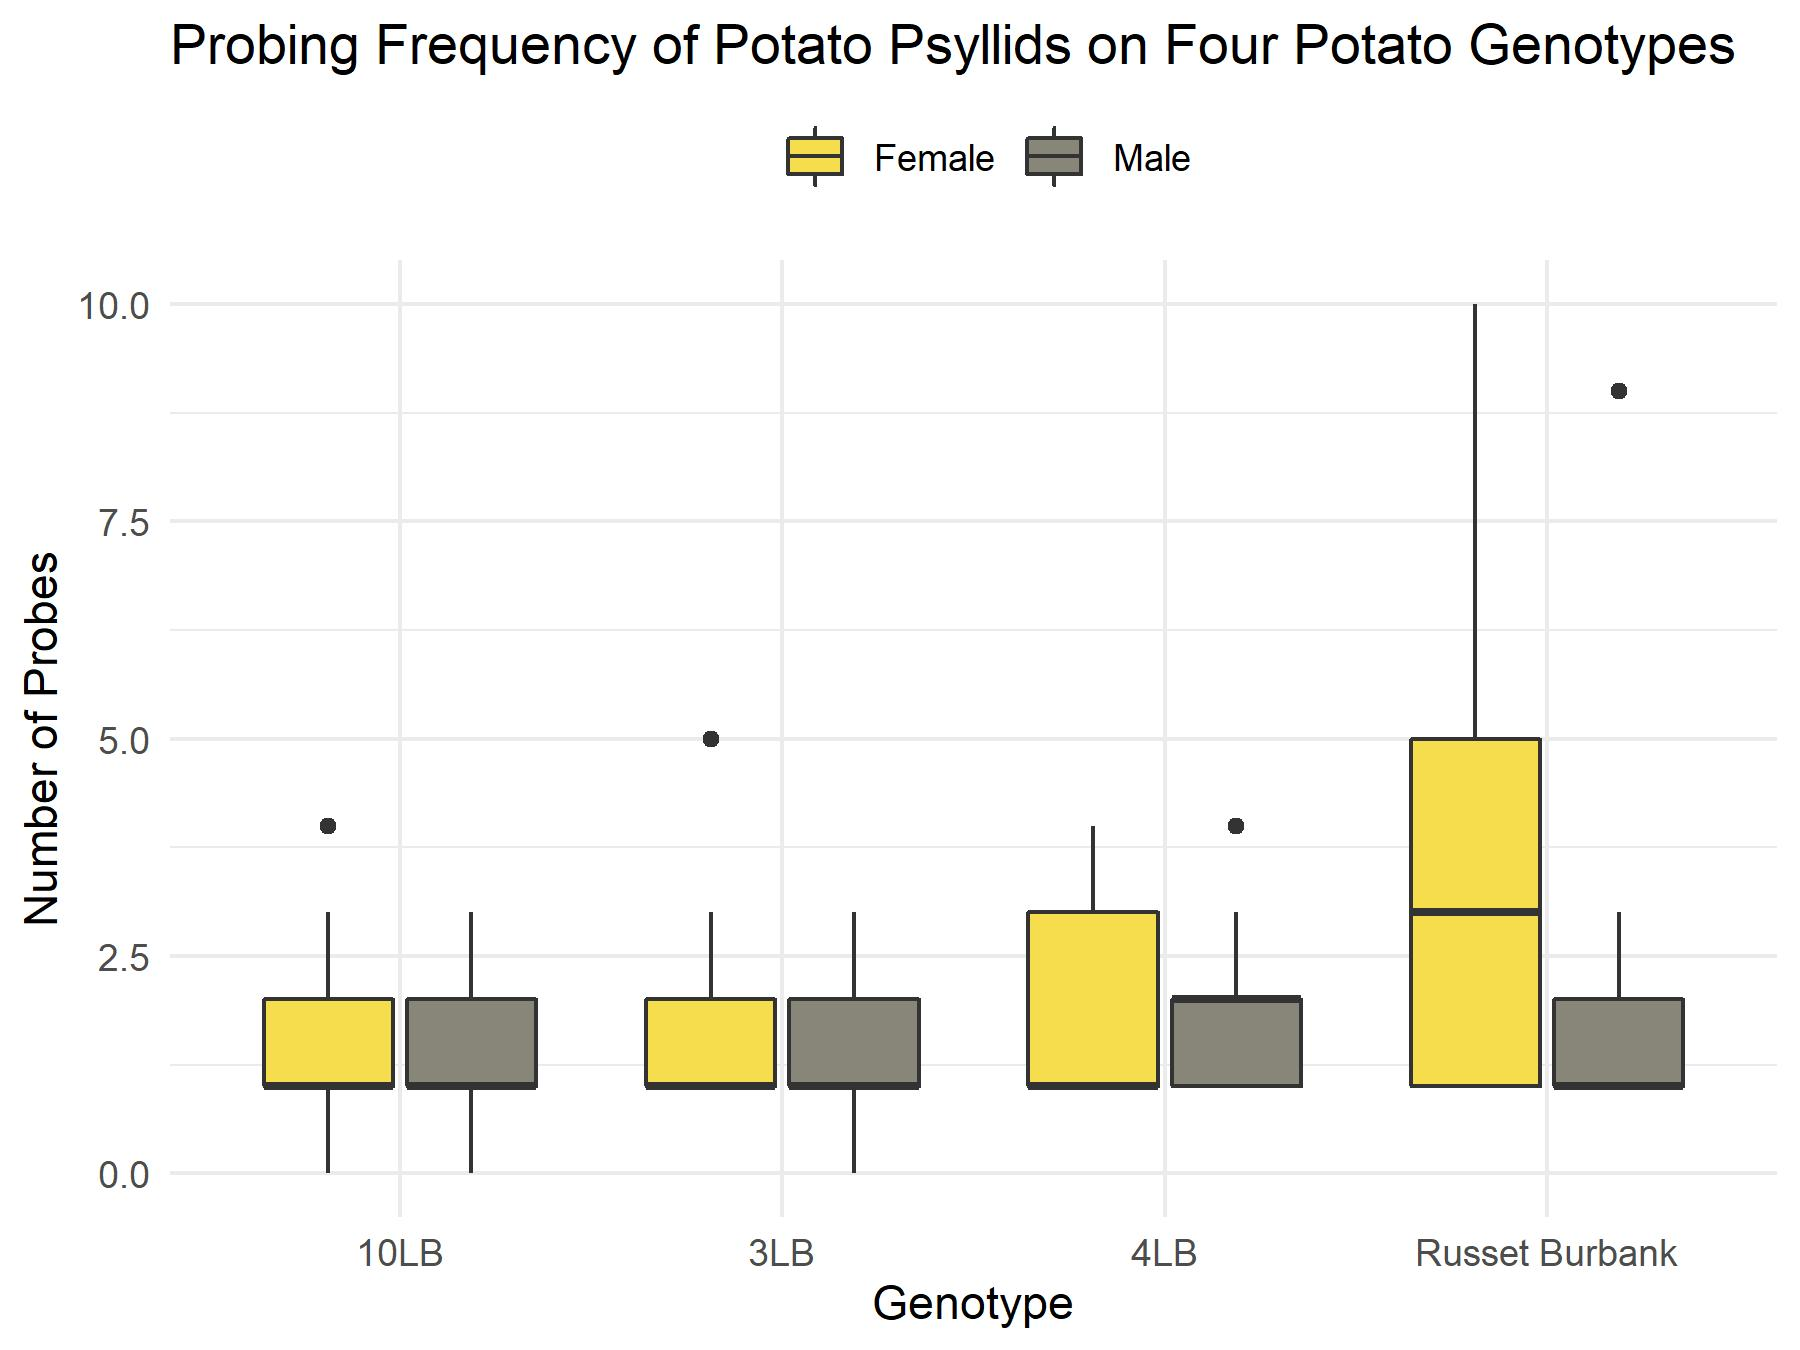
\includegraphics[scale=1]{fig_3.jpg}
%	\caption[Boxplot of probing incidence]{Boxplots of psyllid probing frequency during 300 second recordings on different genotypes}
%	\label{fig:fig_3}
%\end{figure}
%
%%Boxplot of probing duration
%\begin{figure}[!htbp]
%	\centering
%	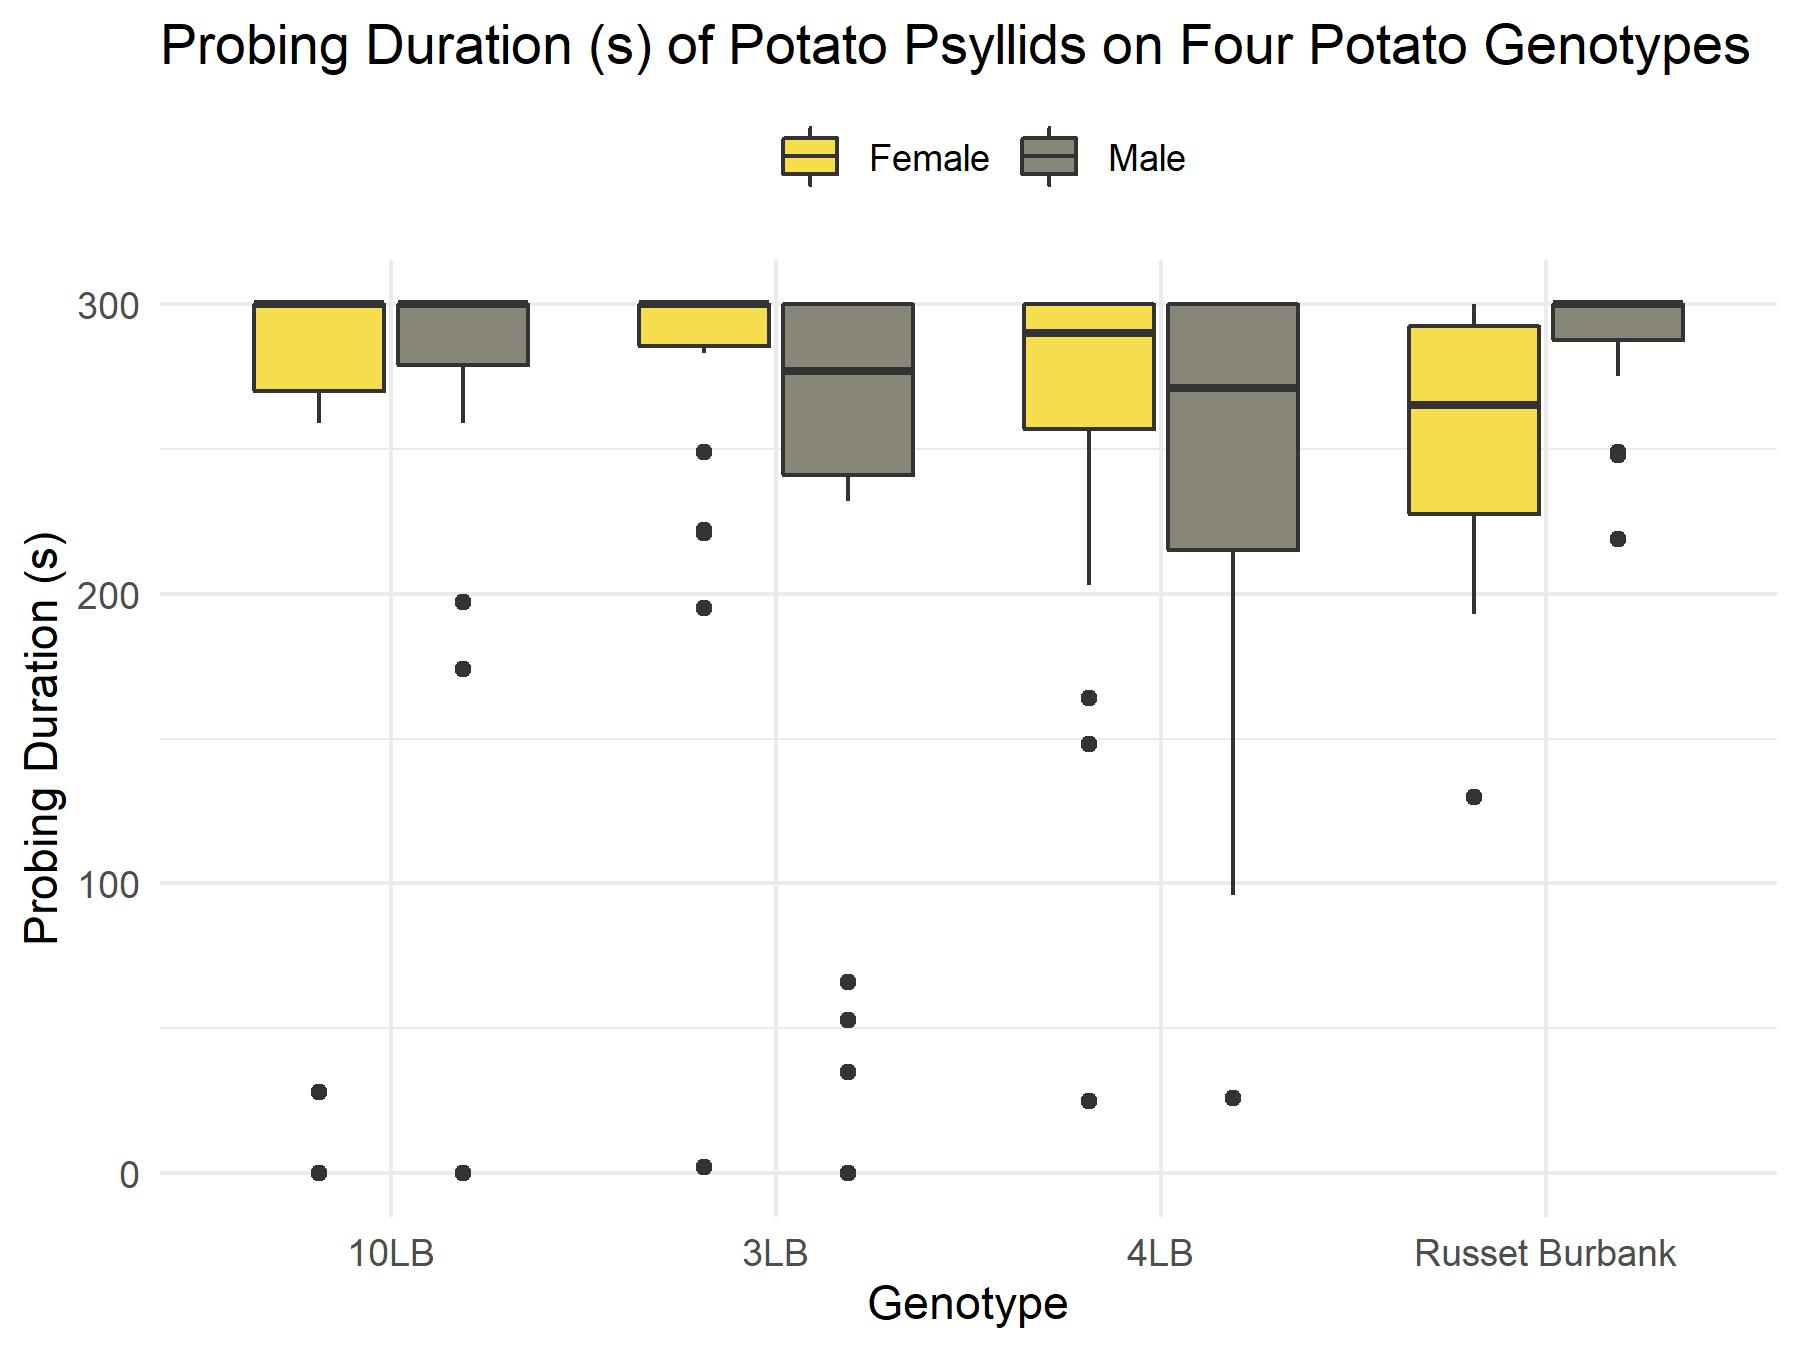
\includegraphics[scale=1]{fig_4.jpg}
%	\caption[Boxplot of probing duration]{Boxplots of psyllids probing duration during 300 second recordings on different genotypes}
%	\label{fig:fig_4}
%\end{figure}
%
%
%%Boxplot of walking incidence
%\begin{figure}[!htbp]
%	\centering
%	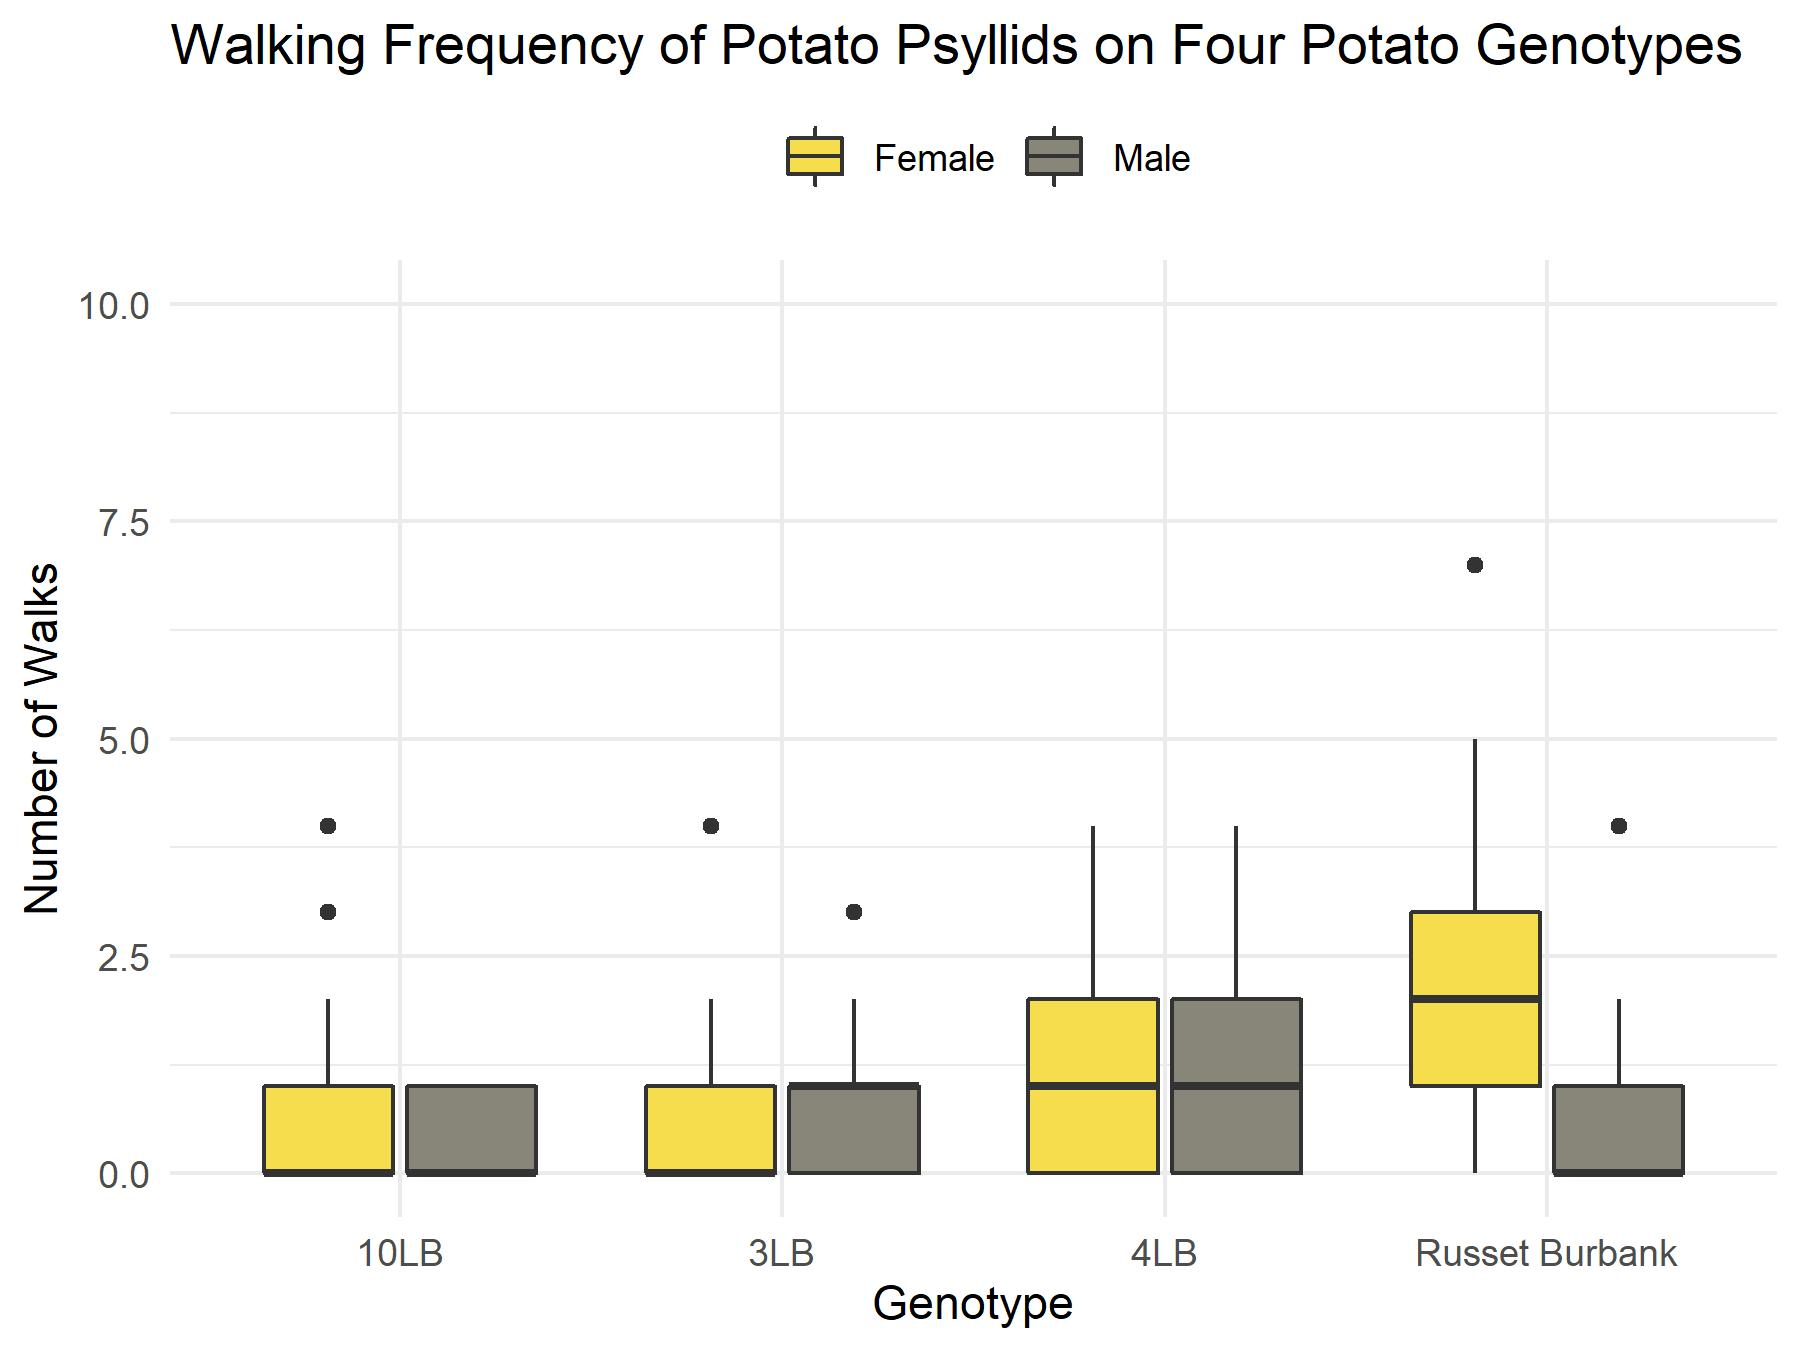
\includegraphics[scale=1]{fig_5.jpg}
%	\caption[Boxplot of walking incidence]{Boxplots of psyllid walking frequency during 300 second recordings on different genotypes}
%	\label{fig:fig_5}
%\end{figure}
%
%
%%Boxplot of walking duration
%\begin{figure}[!htbp]
%	\centering
%	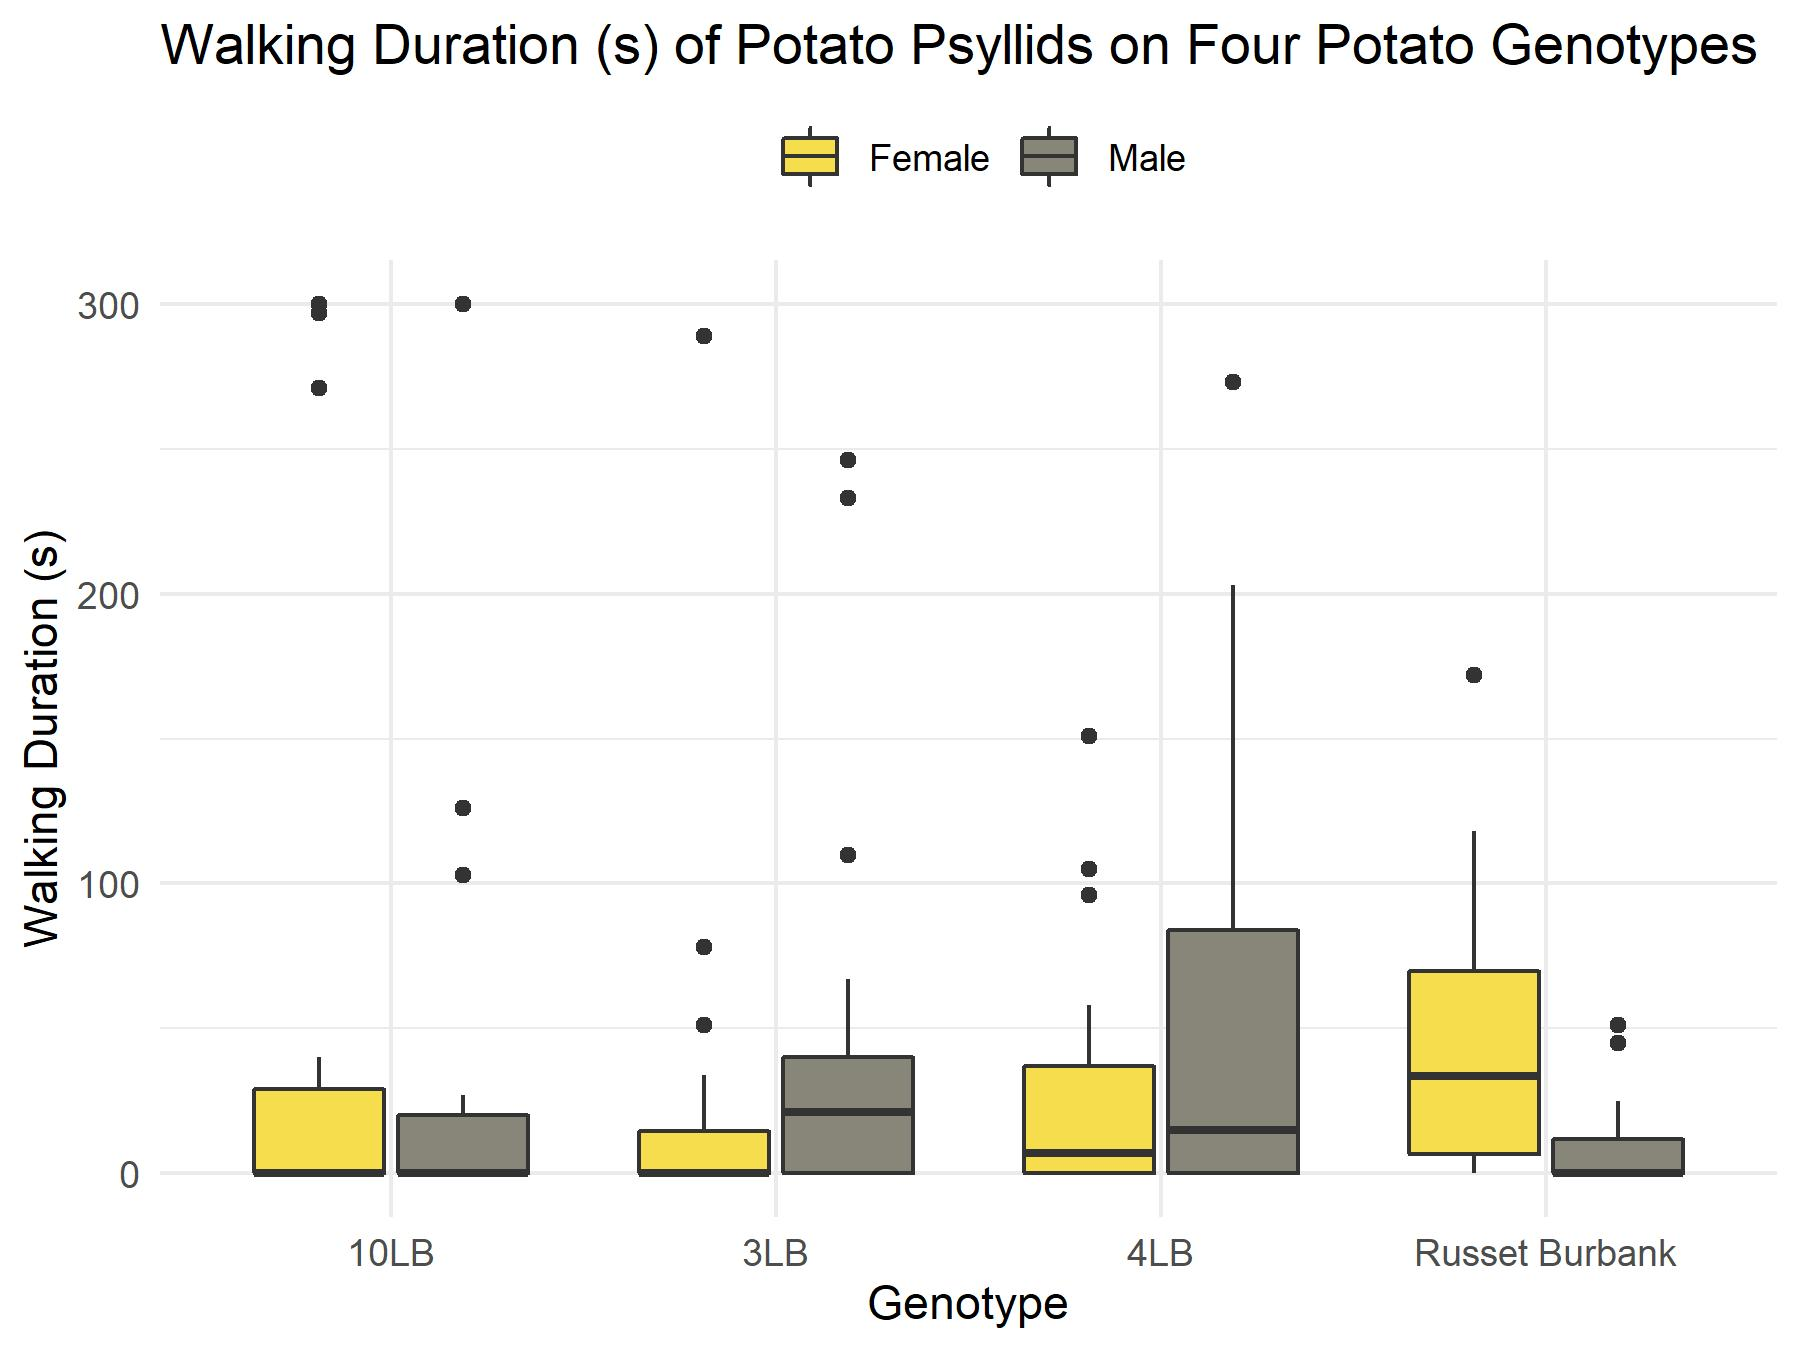
\includegraphics[scale=1]{fig_6.jpg}
%	\caption[Boxplot of walking duration]{Boxplots of psyllid walking duration during 300 second recordings on different genotypes}
%	\label{fig:fig_6}
%\end{figure}
%
%%Boxplot of egg production per period
%\begin{figure}[!htbp]
%	\centering
%	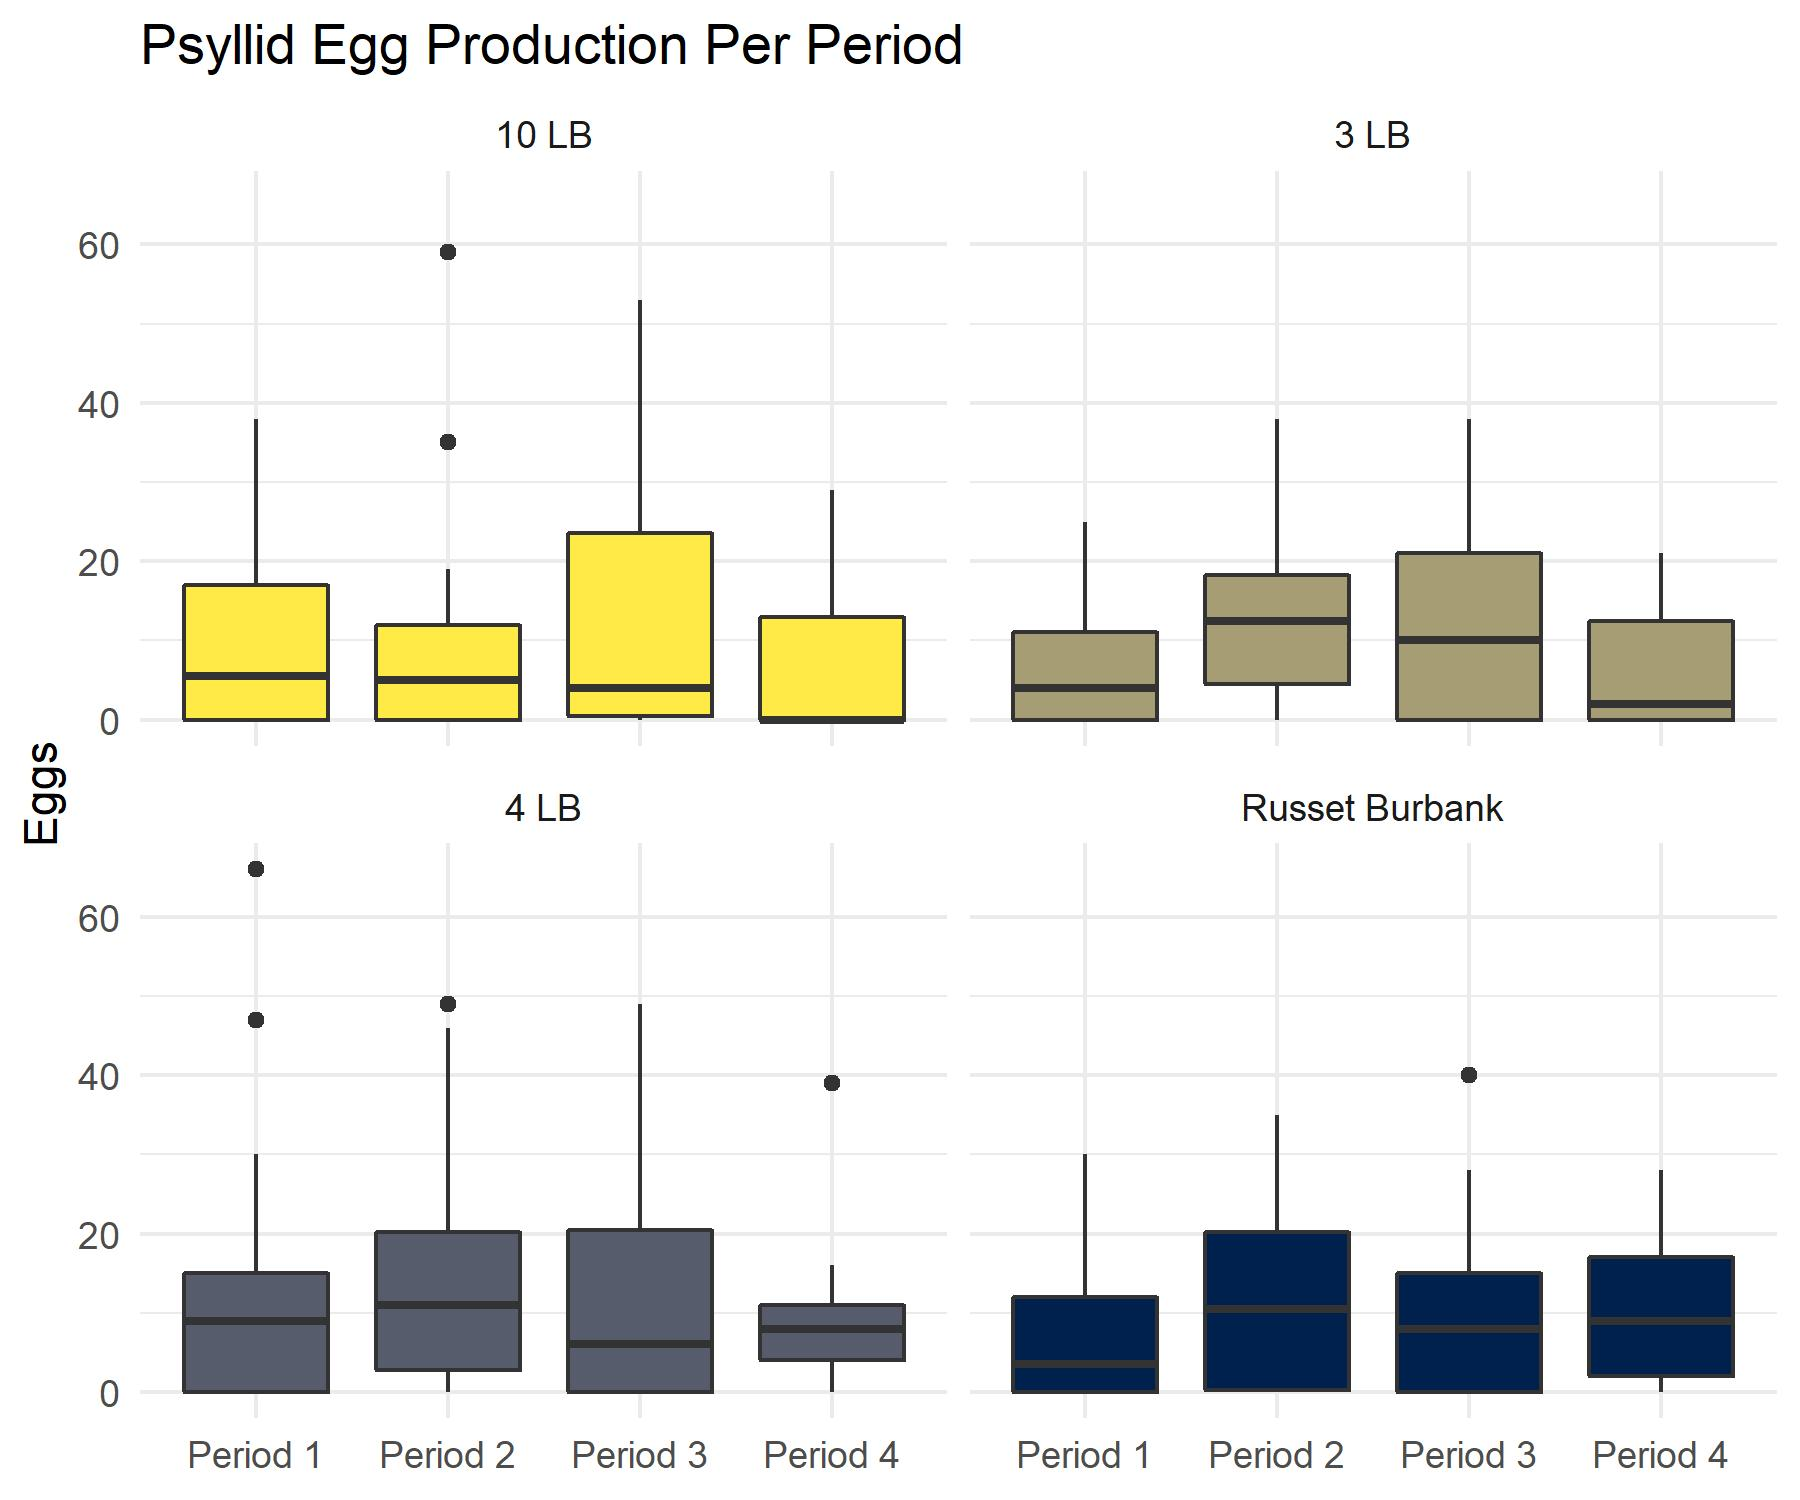
\includegraphics[scale=1]{fig_11.jpg}
%	\caption[Boxplots of psyllid egg production per period on four different genotypes]{Boxplots of psyllid egg production per period on four different genotypes. A mating pair of female and male psyllids were placed on a caged plant for six to eight days after which the male was removed. The remaining female was transferred every four days to a new plant of the same genotype until 12 more days had elapsed. Eggs were counted after each transfer.}
%	\label{fig:fig_11}
%\end{figure}

%%Boxplot of nymphs counted per period
%\begin{figure}[!htbp]
%	\centering
%	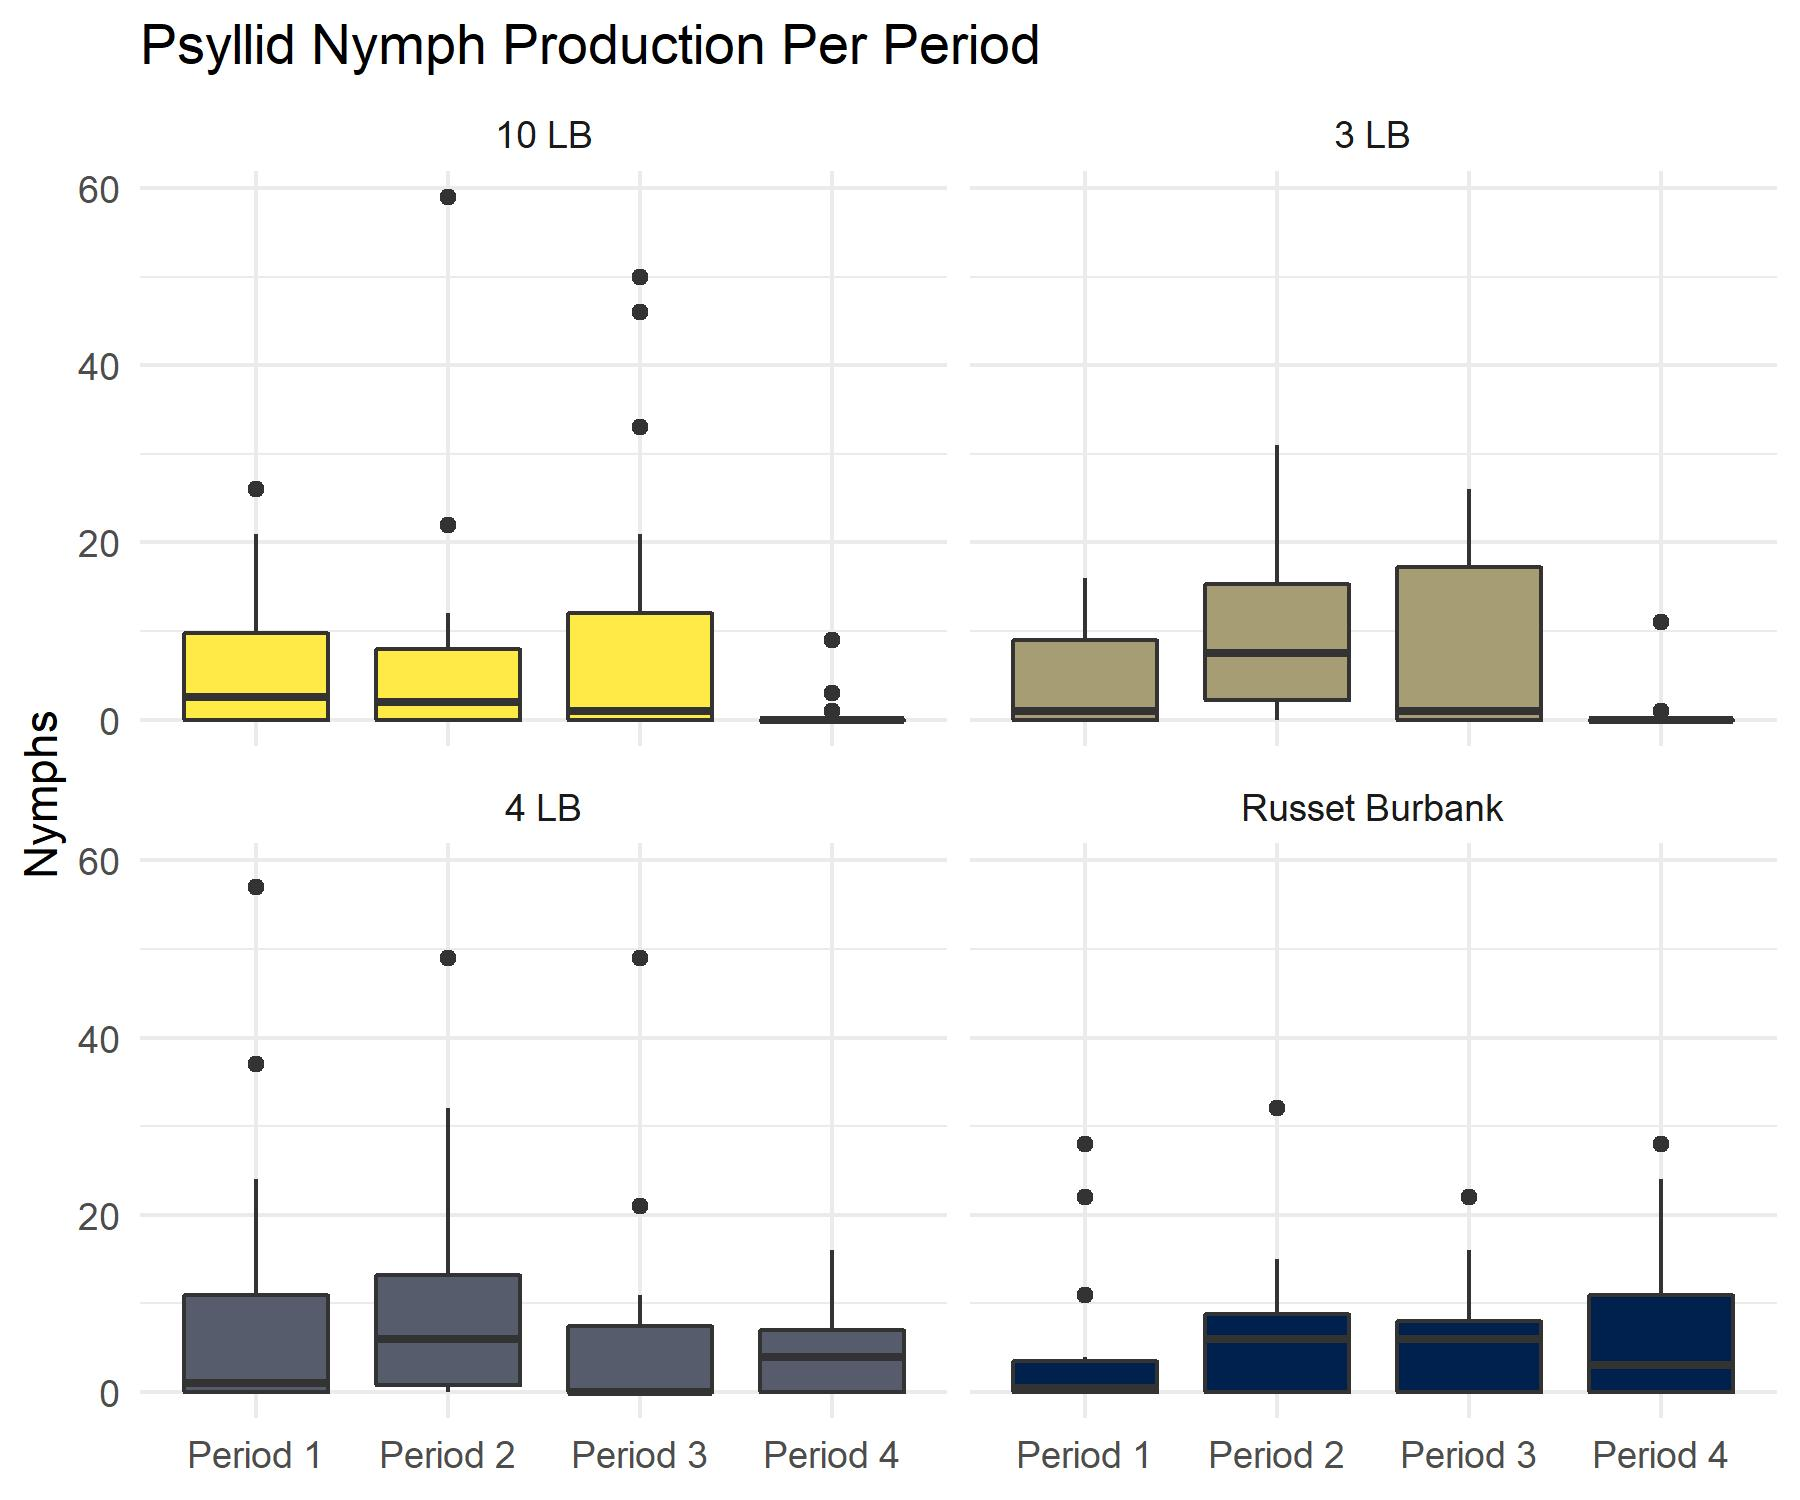
\includegraphics[scale=1]{fig_12.jpg}
%	\caption[Boxplots of psyllid nymphs counted per period on four different genotypes]{Boxplots of psyllid nymphs counted per period on four different genotypes. A mating pair of female and male psyllids were placed on a caged plant for six to eight days after which the male was removed. The remaining female was transferred every four days to a new plant of the same genotype until 12 more days had elapsed. Nymphs were counted after transfer and during the week after female transfer. Nymphs were removed as counted.}
%	\label{fig:fig_12}
%\end{figure}
%
%%Boxplot of egg fertility per period
%\begin{figure}[!htbp]
%	\centering
%	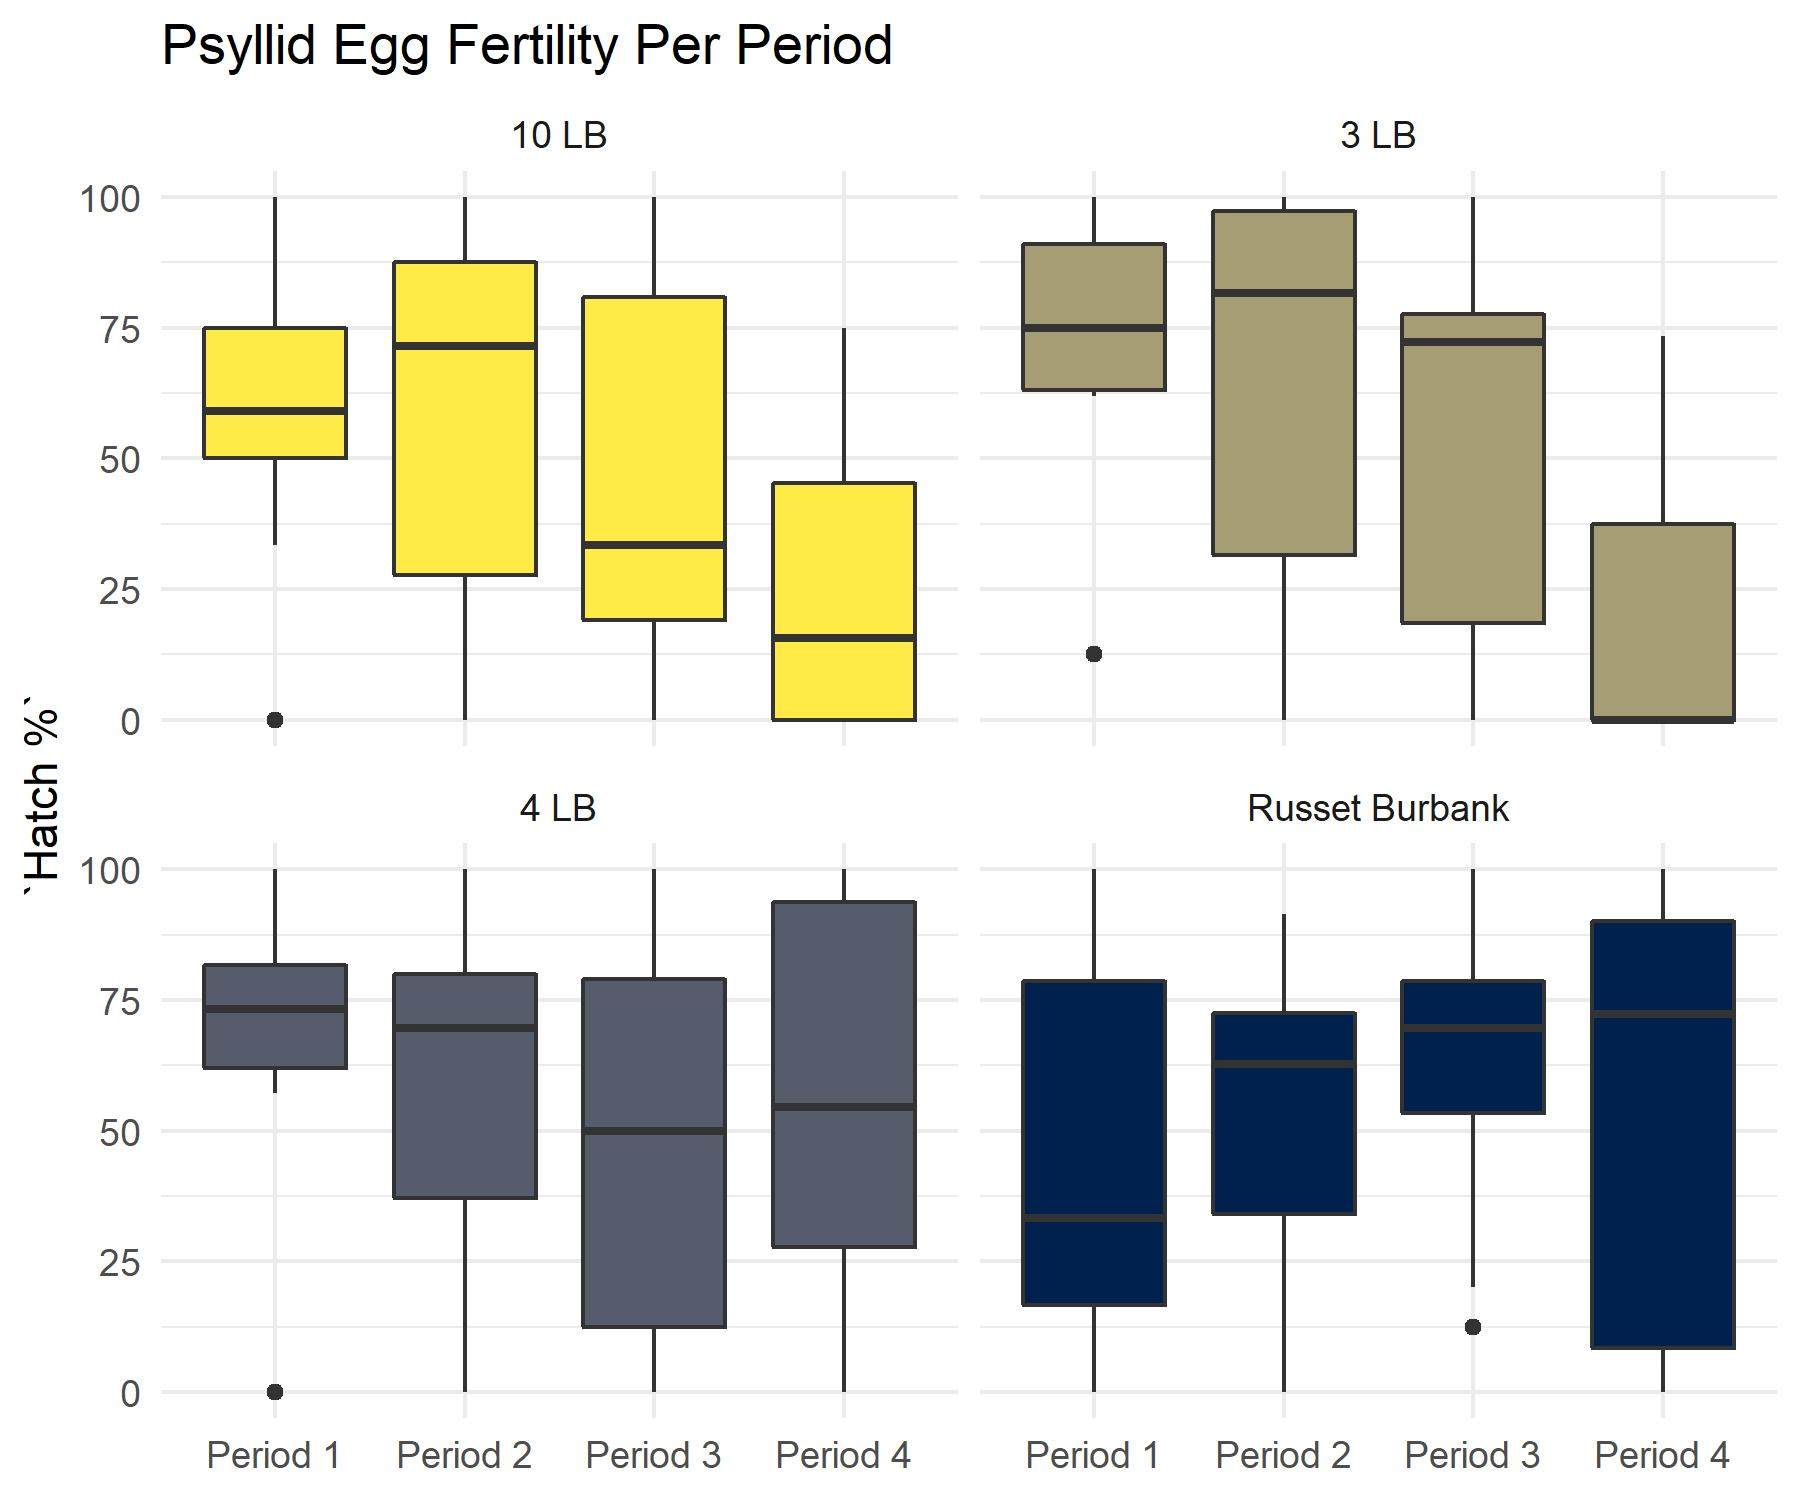
\includegraphics[scale=1]{fig_13.jpg}
%	\caption[Boxplots of psyllid fertility per period on four different genotypes]{Boxplots of psyllid fertility per period on four different genotypes. A mating pair of female and male psyllids were placed on a caged plant for six to eight days after which the male was removed. The remaining female was transferred every four days to a new plant of the same genotype until 12 more days had elapsed. Egg fertility was calculated as the percentage of nymphs hatched from the total number of eggs laid.}
%	\label{fig:fig_13}
%\end{figure}

%\section{R session information:}
%\label{sec:session}
%\begin{itemize}\raggedright
%	\item R version 3.5.1 (2018-07-02), \verb|x86_64-w64-mingw32|
%	\item Locale: \verb|LC_COLLATE=English_United States.1252|, \verb|LC_CTYPE=English_United States.1252|, \verb|LC_MONETARY=English_United States.1252|, \verb|LC_NUMERIC=C|, \verb|LC_TIME=English_United States.1252|
%	\item Running under: \verb|Windows >= 8 x64 (build 9200)|
%	\item Matrix products: default
%	\item Base packages: base, datasets, graphics, grDevices, methods, stats, utils
%	\item Other packages: bindrcpp~0.2.2, car~3.0-2, carData~3.0-2, dplyr~0.7.7,
%	emmeans~1.2.4, fitdistrplus~1.0-11, forcats~0.3.0, ggplot2~3.0.0, lme4~1.1-18-1,
%	lsei~1.2-0, MASS~7.3-50, Matrix~1.2-14, multcompView~0.1-7, npsurv~0.4-0,
%	optimx~2018-7.10, pastecs~1.3.21, purrr~0.2.5, pwr~1.2-2, readr~1.1.1, stringr~1.3.1,
%	survival~2.42-3, tibble~1.4.2, tidyr~0.8.1, tidyverse~1.2.1, viridis~0.5.1,
%	viridisLite~0.3.0, writexl~1.0
%	\item Loaded via a namespace (and not attached): abind~1.4-5, assertthat~0.2.0,
%	backports~1.1.2, bindr~0.1.1, boot~1.3-20, broom~0.5.0, cellranger~1.1.0, cli~1.0.1,
%	codetools~0.2-15, colorspace~1.3-2, compiler~3.5.1, crayon~1.3.4, curl~3.2,
%	data.table~1.11.8, digest~0.6.18, estimability~1.3, foreign~0.8-70, glue~1.3.0,
%	grid~3.5.1, gridExtra~2.3, gtable~0.2.0, haven~1.1.2, hms~0.4.2, httr~1.3.1,
%	jsonlite~1.5, labeling~0.3, lattice~0.20-35, lazyeval~0.2.1, lubridate~1.7.4,
%	magrittr~1.5, minqa~1.2.4, modelr~0.1.2, multcomp~1.4-8, munsell~0.5.0, mvtnorm~1.0-8,
%	nlme~3.1-137, nloptr~1.2.1, numDeriv~2016.8-1, openxlsx~4.1.0, pillar~1.3.0,
%	pkgconfig~2.0.2, plyr~1.8.4, R6~2.3.0, Rcpp~0.12.19, readxl~1.1.0, rio~0.5.10,
%	rlang~0.2.2, rstudioapi~0.8, rvest~0.3.2, sandwich~2.5-0, scales~1.0.0, splines~3.5.1,
%	stringi~1.2.4, TH.data~1.0-9, tidyselect~0.2.5, tools~3.5.1, withr~2.1.2, xml2~1.2.0,
%	xtable~1.8-3, yaml~2.2.0, zip~1.0.0, zoo~1.8-4
%\end{itemize}

% --------------------------------------------------------------------------
% -- References --
\clearpage
\printbibliography
\renewcommand\bibname{References Cited} % Relabels bibliography title as "REFERENCES"
\addcontentsline{toc}{chapter}{\textsc{\bibname}} % Adds to table of contents

% --------------------------------------------------------------------------


\end{document}

% ** DO NOT PUT ANYTHING AFTER THE END OF THE DOCUMENT! **




